\documentclass[aspectratio=169, 11pt]{beamer}

% ── Theme: the shared course style of Chapter 1.1 ──
\usetheme{default}
\usepackage[T1]{fontenc}
\usepackage{lmodern}
\usepackage{appendixnumberbeamer}

\usepackage{amsmath, amssymb, amsfonts}
\usepackage{booktabs}
\usepackage{listings}
\usepackage{xcolor}
\usepackage{tikz}
\usetikzlibrary{arrows.meta, positioning, shapes.geometric, fit}
\usepackage{graphicx}
\usepackage{multicol}
\graphicspath{{experiments/figures/}}

% ── Course colours and slide layout (as in Chapter 1.1) ──
\definecolor{FEMnavy}{HTML}{17365D}
\definecolor{FEMblue}{HTML}{2B6CB0}
\definecolor{FEMteal}{HTML}{1597A5}
\definecolor{FEMorange}{HTML}{D7653B}
\definecolor{FEMlight}{HTML}{F4F7FA}
\definecolor{FEMgray}{HTML}{5C6F82}
\definecolor{FEMpale}{HTML}{EAF7F9}
\definecolor{FEMcream}{HTML}{FFF4EA}
\setbeamercolor{normal text}{fg=FEMnavy,bg=white}
\setbeamercolor{structure}{fg=FEMblue}
\setbeamercolor{frametitle}{fg=white,bg=FEMnavy}
\setbeamercolor{title}{fg=white}
\setbeamercolor{block title}{fg=white,bg=FEMblue}
\setbeamercolor{block body}{fg=FEMnavy,bg=FEMlight}
\setbeamercolor{alerted text}{fg=FEMorange}
\setbeamercolor{block title alerted}{fg=white,bg=FEMorange}
\setbeamercolor{block body alerted}{fg=FEMnavy,bg=FEMcream}
\setbeamercolor{block title example}{fg=white,bg=FEMteal}
\setbeamercolor{block body example}{fg=FEMnavy,bg=FEMpale}
\setbeamertemplate{navigation symbols}{}
\setbeamertemplate{itemize item}{\color{FEMteal}$\blacktriangleright$}
\setbeamertemplate{itemize subitem}{\color{FEMteal}$\bullet$}
\setbeamertemplate{frametitle}{\nointerlineskip\begin{beamercolorbox}[wd=\paperwidth,ht=.82cm,dp=.25cm,leftskip=.55cm]{frametitle}\usebeamerfont{frametitle}\insertframetitle\end{beamercolorbox}}
\setbeamertemplate{footline}{\leavevmode\hbox{\begin{beamercolorbox}[wd=.82\paperwidth,ht=2.6ex,dp=1.1ex,leftskip=.55cm]{author in head/foot}\color{FEMgray}\scriptsize Introduction to FEniCS -- Part I\end{beamercolorbox}\begin{beamercolorbox}[wd=.18\paperwidth,ht=2.6ex,dp=1.1ex,rightskip=.55cm plus1fil]{date in head/foot}\color{FEMgray}\scriptsize\hfill\insertframenumber/\inserttotalframenumber\end{beamercolorbox}}}
\setbeamersize{text margin left=.65cm,text margin right=.65cm}
\setbeamerfont{frametitle}{size=\Large,series=\bfseries}
\setbeamerfont{block title}{size=\normalsize,series=\bfseries}

% Title and divider slides in the style of the Chapter 1.1 title page.
\newcommand{\meshmotif}{%
\begin{scope}[shift={(current page.south east)},x=1cm,y=1cm]
\foreach \x in {-6,-4.7,-3.4,-2.1,-.8}{\foreach \y in {.1,1.4,2.7,4,5.3,6.6}{
\draw[white,opacity=.10] (\x,\y) rectangle ++(1.3,1.3);
\draw[white,opacity=.10] (\x,\y)--++(1.3,1.3);}}
\end{scope}}
% #1 kicker line, #2 bottom line
\newcommand{\coursetitleframe}[2]{%
\begin{frame}[plain]
\begin{tikzpicture}[remember picture,overlay]
\fill[FEMnavy] (current page.south west) rectangle (current page.north east);
\meshmotif
\node[anchor=west,text width=12.7cm,align=left] at ([xshift=.85cm,yshift=.55cm]current page.west) {
{\color{FEMteal!70!white}\large\bfseries #1}\\[7mm]
{\color{white}\fontsize{29}{34}\selectfont\bfseries\inserttitle}\\[5mm]
{\color{white!80}\Large\insertsubtitle}\\[6mm]
{\color{white!70}\large\insertauthor}};
\node[anchor=south west,text=white!70] at ([xshift=.85cm,yshift=.72cm]current page.south west) {#2};
\end{tikzpicture}
\end{frame}}
% #1 kicker line (may be empty), #2 title
\newcommand{\dividerframe}[2]{%
\begin{frame}[plain]
\begin{tikzpicture}[remember picture,overlay]
\fill[FEMnavy] (current page.south west) rectangle (current page.north east);
\meshmotif
\node[anchor=west,text width=12.7cm,align=left] at ([xshift=.85cm]current page.west) {
\ifx\relax#1\relax\else{\color{FEMteal!70!white}\large\bfseries #1}\\[6mm]\fi
{\color{white}\fontsize{26}{31}\selectfont\bfseries\hyphenpenalty=10000\exhyphenpenalty=10000 #2\par}};
\end{tikzpicture}
\end{frame}}

% ── Code listing style ──
\colorlet{codebg}{FEMlight}
\definecolor{codegreen}{HTML}{2E7D32}
\colorlet{codeapi}{FEMteal!85!black}   % FEniCS/UFL names
\colorlet{codeorange}{FEMorange}
\colorlet{codegray}{FEMgray}
\colorlet{codeblue}{FEMblue}

\lstdefinestyle{fenics}{
    language=Python,
    backgroundcolor=\color{codebg},
    basicstyle=\ttfamily\scriptsize,
    keywordstyle=\color{codeblue}\bfseries,
    stringstyle=\color{codegreen},
    commentstyle=\color{codegray}\itshape,
    emphstyle=\color{codeapi}\bfseries,
    emph={FunctionSpace, TrialFunction, TestFunction, Function,
          DirichletBC, Expression, Constant, UnitSquareMesh,
          VectorFunctionSpace, NonlinearVariationalProblem,
          NonlinearVariationalSolver, MixedElement,
          FiniteElement, solve, assemble, plot, errornorm,
          project, derivative, interpolate, grad, div, dot,
          inner, dx, ds},
    morekeywords={[2]mesh, V, u, v, a, L, bc, f, u_h, u_D, W, Q, p, q},
    keywordstyle={[2]\color{codeorange}},
    numbers=left,
    numberstyle=\tiny\color{codegray},
    numbersep=5pt,
    frame=single,
    rulecolor=\color{FEMblue!20},
    breaklines=true,
    showstringspaces=false,
    tabsize=4,
    xleftmargin=6pt,
    xrightmargin=4pt,
    aboveskip=6pt,
    belowskip=4pt,
}

\lstset{style=fenics}

% ── Metadata ──
\title{Introduction to FEniCS}
\subtitle{From weak forms to working code}
\author{Daniel Fernandez}
\date{}

% ══════════════════════════════════════════════════════════════
\begin{document}
% ══════════════════════════════════════════════════════════════

\coursetitleframe{FINITE ELEMENTS IN PRACTICE\enspace$\cdot$\enspace PART I}{Weak form\quad$\longrightarrow$\quad Python code\quad$\longrightarrow$\quad verified solution}

% ══════════════════════════════════════════════════════════════
\section{Setup}
% ══════════════════════════════════════════════════════════════

% ──────────────────────────────────────────────────────────────
\begin{frame}[fragile]{FEniCS installation}

\textbf{Conda} (Linux/macOS):
\begin{lstlisting}[language=bash, style=fenics]
conda create -n fenicsx-env
conda activate fenicsx-env
conda install -c conda-forge fenics-dolfinx mpich pyvista
conda activate fenicsx-env
\end{lstlisting}

\end{frame}

% ══════════════════════════════════════════════════════════════
\section{Motivation}
% ══════════════════════════════════════════════════════════════

% ──────────────────────────────────────────────────────────────
\begin{frame}{From the weak form to a solver}

Once you have the weak formulation, the implementation needs six steps:

\begin{enumerate}
    \item Write a mesh generator
    \item Implement basis functions
    \item Assemble stiffness/mass matrices
    \item Handle boundary conditions
    \item Solve the linear system
    \item Post-process and visualize
\end{enumerate}

\medskip
\textbf{FEniCS} provides mesh and element tools and assembles the system
from a weak form written in Python.

\end{frame}

% ──────────────────────────────────────────────────────────────
\begin{frame}[fragile]{The weak form in code}

\begin{columns}[T]
\column{0.48\textwidth}
\textbf{On paper:}

Find $u \in V$ such that
\[
  \int_\Omega \nabla u \cdot \nabla v \, dx
  = \int_\Omega f \, v \, dx
  \quad \forall\, v \in \hat{V}
\]

\column{0.48\textwidth}
\textbf{In FEniCS:}

\begin{lstlisting}
u = TrialFunction(V)
v = TestFunction(V)

a = dot(grad(u), grad(v)) * dx
L = f * v * dx

solve(a == L, u_h, bc)
\end{lstlisting}
\end{columns}

\bigskip
\begin{center}
The two integrals translate directly into UFL expressions.
\end{center}

\small
\textbf{Strength:} Write the weak form and let FEniCS assemble it.
\\
\textbf{Trade-off:} Custom assembly requires working below this interface.
\\
\textbf{Note:} $hp$-adaptivity is not directly ``implemented'' in FEniCS.

\end{frame}

% ──────────────────────────────────────────────────────────────
\section{Mathematical background}
% ══════════════════════════════════════════════════════════════

% ──────────────────────────────────────────────────────────────
\begin{frame}{A brief FEM recap}

Given a PDE: $-\Delta u = f$ in $\Omega$, $u = g$ on $\partial\Omega$.

\bigskip

\begin{enumerate}
    \item \textbf{Weak form:}
        Find $u \in H_g^1(\Omega)$ s.t.\ $a(u,v) = L(v)$ $\forall v \in H_0^1(\Omega)$
    \[
      a(u,v) = \int_\Omega \nabla u \cdot \nabla v \, dx,
      \quad
      L(v) = \int_\Omega f \, v \, dx
    \]

          \item \textbf{Discretize:} Choose finite-dimensional
              $V_h^g \subset H_g^1(\Omega)$ and $V_{h,0} \subset H_0^1(\Omega)$
              (piecewise polynomials on a mesh $\mathcal{T}_h$), and write
              $u_h = g_h + w_h$ with $w_h \in V_{h,0}$.
              Dirichlet data is imposed by interpolating $g$ on boundary DOFs.

    \item \textbf{Assemble:} Build stiffness matrix $A_{ij} = a(\phi_j, \phi_i)$
          and load vector $b_i = L(\phi_i)$

    \item \textbf{Solve:} $A \mathbf{u} = \mathbf{b}$
\end{enumerate}

\bigskip
You choose the mesh, elements, and solver; FEniCS assembles the symbolic forms.
\end{frame}

% ──────────────────────────────────────────────────────────────
\begin{frame}{Math objects $\to$ FEniCS objects}

\scriptsize
\begin{center}
\renewcommand{\arraystretch}{1.4}
\begin{tabular}{lll}
\toprule
\textbf{Mathematics} & \textbf{FEniCS class} & \textbf{Code} \\
\midrule
Mesh $\mathcal{T}_h$ & \texttt{Mesh} & \texttt{UnitSquareMesh(n, n)} \\
Space $V_h$ & \texttt{FunctionSpace} & \texttt{FunctionSpace(mesh, 'P', k)} \\
Trial function $u$ & \texttt{TrialFunction} & \texttt{u = TrialFunction(V)} \\
Test function $v$ & \texttt{TestFunction} & \texttt{v = TestFunction(V)} \\
Solution $u_h$ & \texttt{Function} & \texttt{u\_h = Function(V)} \\
$g$ (boundary data) & \texttt{Expression} & \texttt{Expression('x[0]*x[0]', ...)} \\
$a(u,v)$ & UFL form & \texttt{dot(grad(u),grad(v))*dx} \\
$L(v)$ & UFL form & \texttt{f*v*dx} \\
BC: $u|_{\partial\Omega}=g$ & \texttt{DirichletBC} & \texttt{DirichletBC(V, g, bdry)} \\
\bottomrule
\end{tabular}
\end{center}

\end{frame}

% ══════════════════════════════════════════════════════════════
\section{Demo: Poisson equation}
% ══════════════════════════════════════════════════════════════

% ──────────────────────────────────────────────────────────────
\dividerframe{EXAMPLE 1}{Poisson equation with a known solution}

% ──────────────────────────────────────────────────────────────
\begin{frame}{Problem statement}

\begin{block}{Poisson equation with known exact solution}
\[
    -\Delta u = -6 \quad \text{in } \Omega = [0,1]^2
\]
\[
  u = 1 + x^2 + 2y^2 \quad \text{on } \partial\Omega
\]
\end{block}

\medskip
Exact solution: $u(x,y) = 1 + x^2 + 2y^2$.

\medskip
\textbf{Why this problem?}
\begin{itemize}
    \item Polynomial exact solution $\Rightarrow$ we can verify convergence rates
    \item $P_2$ elements should give machine-precision accuracy (why?)
\end{itemize}

\end{frame}

% ──────────────────────────────────────────────────────────────
\begin{frame}[fragile]{Step 1: mesh and function space}

\begin{columns}[T]
\column{0.49\textwidth}
\textbf{FEniCS}
\begin{lstlisting}[basicstyle=\ttfamily\tiny]
from fenics import *

mesh = UnitSquareMesh(8, 8)
V = FunctionSpace(mesh, 'P', 1)
\end{lstlisting}

\column{0.49\textwidth}
\textbf{FEniCSx}
\begin{lstlisting}[basicstyle=\ttfamily\tiny]
from mpi4py import MPI
from dolfinx import fem, mesh

msh = mesh.create_unit_square(
    MPI.COMM_WORLD, 8, 8)
V = fem.functionspace(
    msh, ("Lagrange", 1))
\end{lstlisting}
\end{columns}

\medskip
\begin{itemize}
\small
\item Same mathematical setup, with updated object names and constructors in FEniCSx.
\item Discretization choice: \texttt{("Lagrange", k)} means $P_k$ elements
    (e.g. $P_1$ linear, $P_2$ quadratic); DG and mixed spaces are also available.
\item Other mesh choices: \texttt{UnitCubeMesh}, \texttt{RectangleMesh}, \texttt{BoxMesh},
      unstructured meshes from Gmsh, and imported \texttt{XDMF}/\texttt{XML} meshes.
\end{itemize}

\end{frame}

% ──────────────────────────────────────────────────────────────
\begin{frame}[fragile]{Step 2: boundary conditions}

\begin{columns}[T]
\column{0.49\textwidth}
\textbf{FEniCS}
\begin{lstlisting}[basicstyle=\ttfamily\tiny]
u_D = Expression(
    '1 + x[0]*x[0] + 2*x[1]*x[1]',
    degree=2)

def boundary(x, on_boundary):
    return on_boundary

bc = DirichletBC(V, u_D, boundary)
\end{lstlisting}

\column{0.49\textwidth}
\textbf{FEniCSx}
\begin{lstlisting}[basicstyle=\ttfamily\tiny]
u_D = fem.Function(V)
u_D.interpolate(
    lambda x: 1 + x[0]*x[0]
    + 2*x[1]*x[1])

tdim = msh.topology.dim
fdim = tdim - 1
msh.topology.create_connectivity(
    fdim, tdim)
boundary_facets = mesh.exterior_
facet_indices(msh.topology)
boundary_dofs = fem.locate_dofs_
topological(V, fdim, boundary_facets)
bc = fem.dirichletbc(u_D, boundary_dofs)
\end{lstlisting}
\end{columns}

\medskip
\begin{itemize}
\footnotesize
\item Neumann BC enters the weak form as a boundary load, e.g. \texttt{+ g*v*ds}.
\item Robin BC splits into bilinear/linear parts,
    e.g. \texttt{+ beta*u*v*ds} and \texttt{+ beta*uR*v*ds}.
\item Use marked boundary measures:
    \texttt{Measure('ds', subdomain\_data=...)} (FEniCS) or
    \texttt{ufl.Measure("ds", domain=msh, subdomain\_data=...)} (FEniCSx).
\end{itemize}

\end{frame}

% ──────────────────────────────────────────────────────────────
\begin{frame}[fragile]{Step 3: variational problem}

\begin{columns}[T]
\column{0.49\textwidth}
\textbf{FEniCS}
\begin{lstlisting}[basicstyle=\ttfamily\tiny]
u = TrialFunction(V)
v = TestFunction(V)
f = Constant(-6.0)

a = dot(grad(u), grad(v))*dx
L = f*v*dx
\end{lstlisting}

\column{0.49\textwidth}
\textbf{FEniCSx}
\begin{lstlisting}[basicstyle=\ttfamily\tiny]
import ufl
from dolfinx import default_scalar_type

u = ufl.TrialFunction(V)
v = ufl.TestFunction(V)
f = fem.Constant(
    msh, default_scalar_type(-6.0))

a = ufl.dot(ufl.grad(u),
            ufl.grad(v))*ufl.dx
L = f*v*ufl.dx
\end{lstlisting}
\end{columns}

\end{frame}

% ──────────────────────────────────────────────────────────────
\begin{frame}[fragile]{Step 4: solve and analyze}

\begin{columns}[T]
\column{0.49\textwidth}
\textbf{FEniCS}
\begin{lstlisting}[basicstyle=\ttfamily\tiny]
u_h = Function(V)
solve(a == L, u_h, bc)

error_L2 = errornorm(u_D, u_h, 'L2')
error_H1 = errornorm(u_D, u_h, 'H1')
print(f"L2 error: {error_L2:.6e}")
print(f"H1 error: {error_H1:.6e}")

plot(u_h)
plot(mesh)
\end{lstlisting}

\column{0.49\textwidth}
\textbf{FEniCSx}
\begin{lstlisting}[basicstyle=\ttfamily\tiny]
from dolfinx.fem.petsc import LinearProblem

problem = LinearProblem(
    a, L, bcs=[bc],
    petsc_options_prefix="exp1_",
    petsc_options={"ksp_type": "preonly",
                   "pc_type": "lu"})
u_h = problem.solve()

err = fem.form(ufl.inner(u_h-u_D, u_h-u_D)
               * ufl.dx)
E_L2 = np.sqrt(msh.comm.allreduce(
    fem.assemble_scalar(err), op=MPI.SUM))
print(f"L2 error: {E_L2:.6e}")
\end{lstlisting}
\end{columns}

\medskip
\begin{itemize}
\scriptsize
\item Default: legacy \texttt{solve(...)} uses backend defaults (often LU);
      FEniCSx uses PETSc defaults unless \texttt{petsc\_options} are set.
\item Solver families: CG/GMRES/MINRES with ILU/HYPRE/GAMG/MUMPS,
      plus Newton/SNES for nonlinear systems.
\item In inverse settings, add regularization, e.g.
      Tikhonov $\alpha\|m\|^2$ or gradient $\alpha\|\nabla m\|^2$.
\end{itemize}

\end{frame}

% ──────────────────────────────────────────────────────────────
\begin{frame}{Solution and mesh visualization}

\begin{center}
    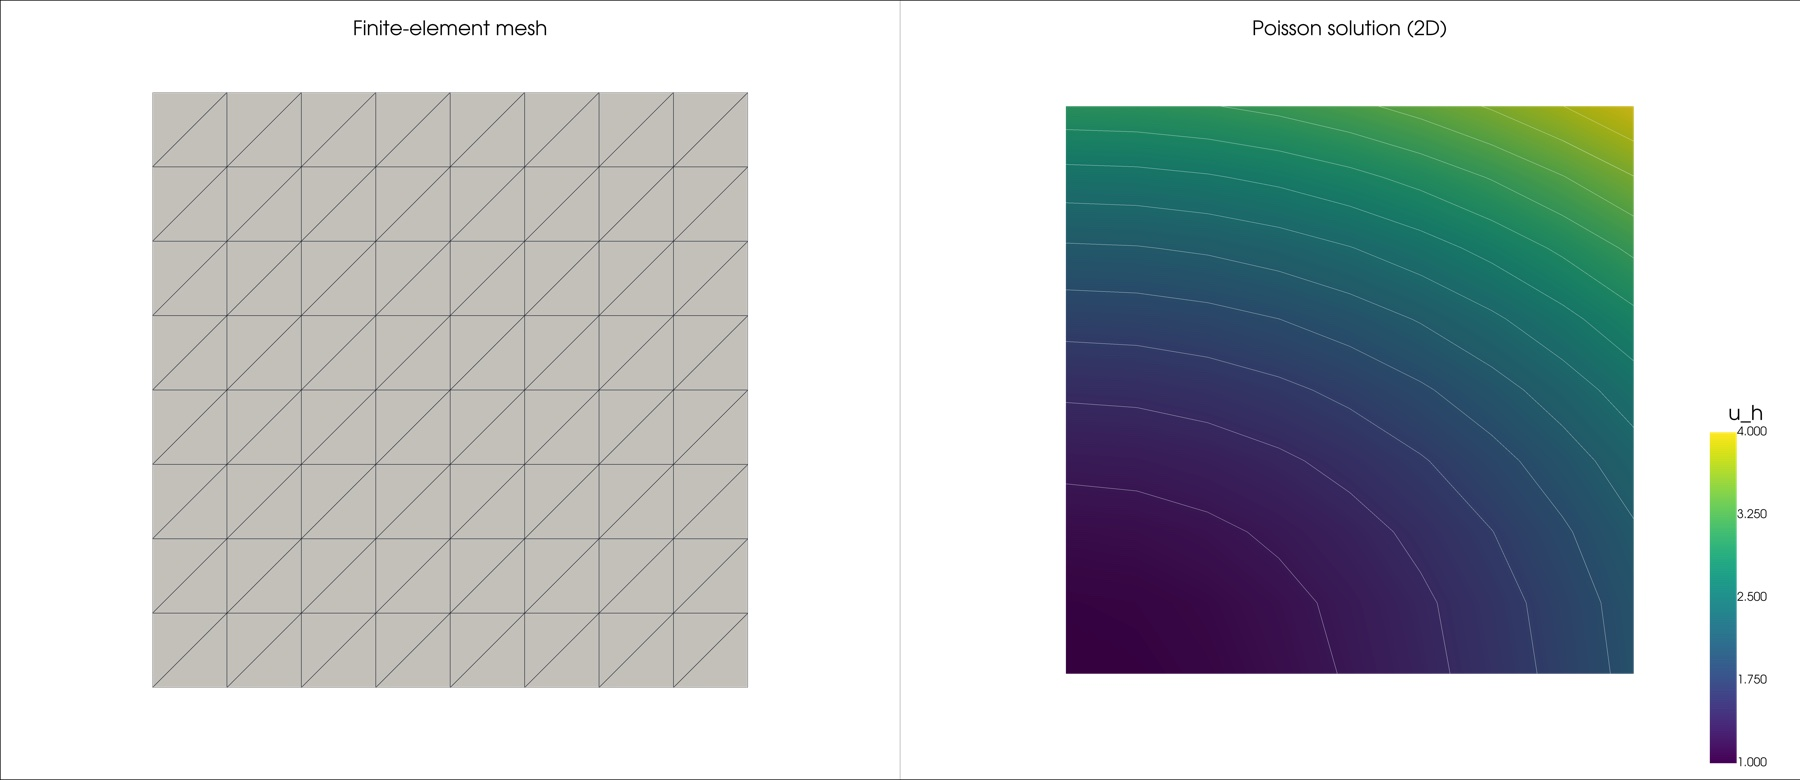
\includegraphics[width=0.495\textwidth]{poisson_solution_slide.jpg}
    \hfill
    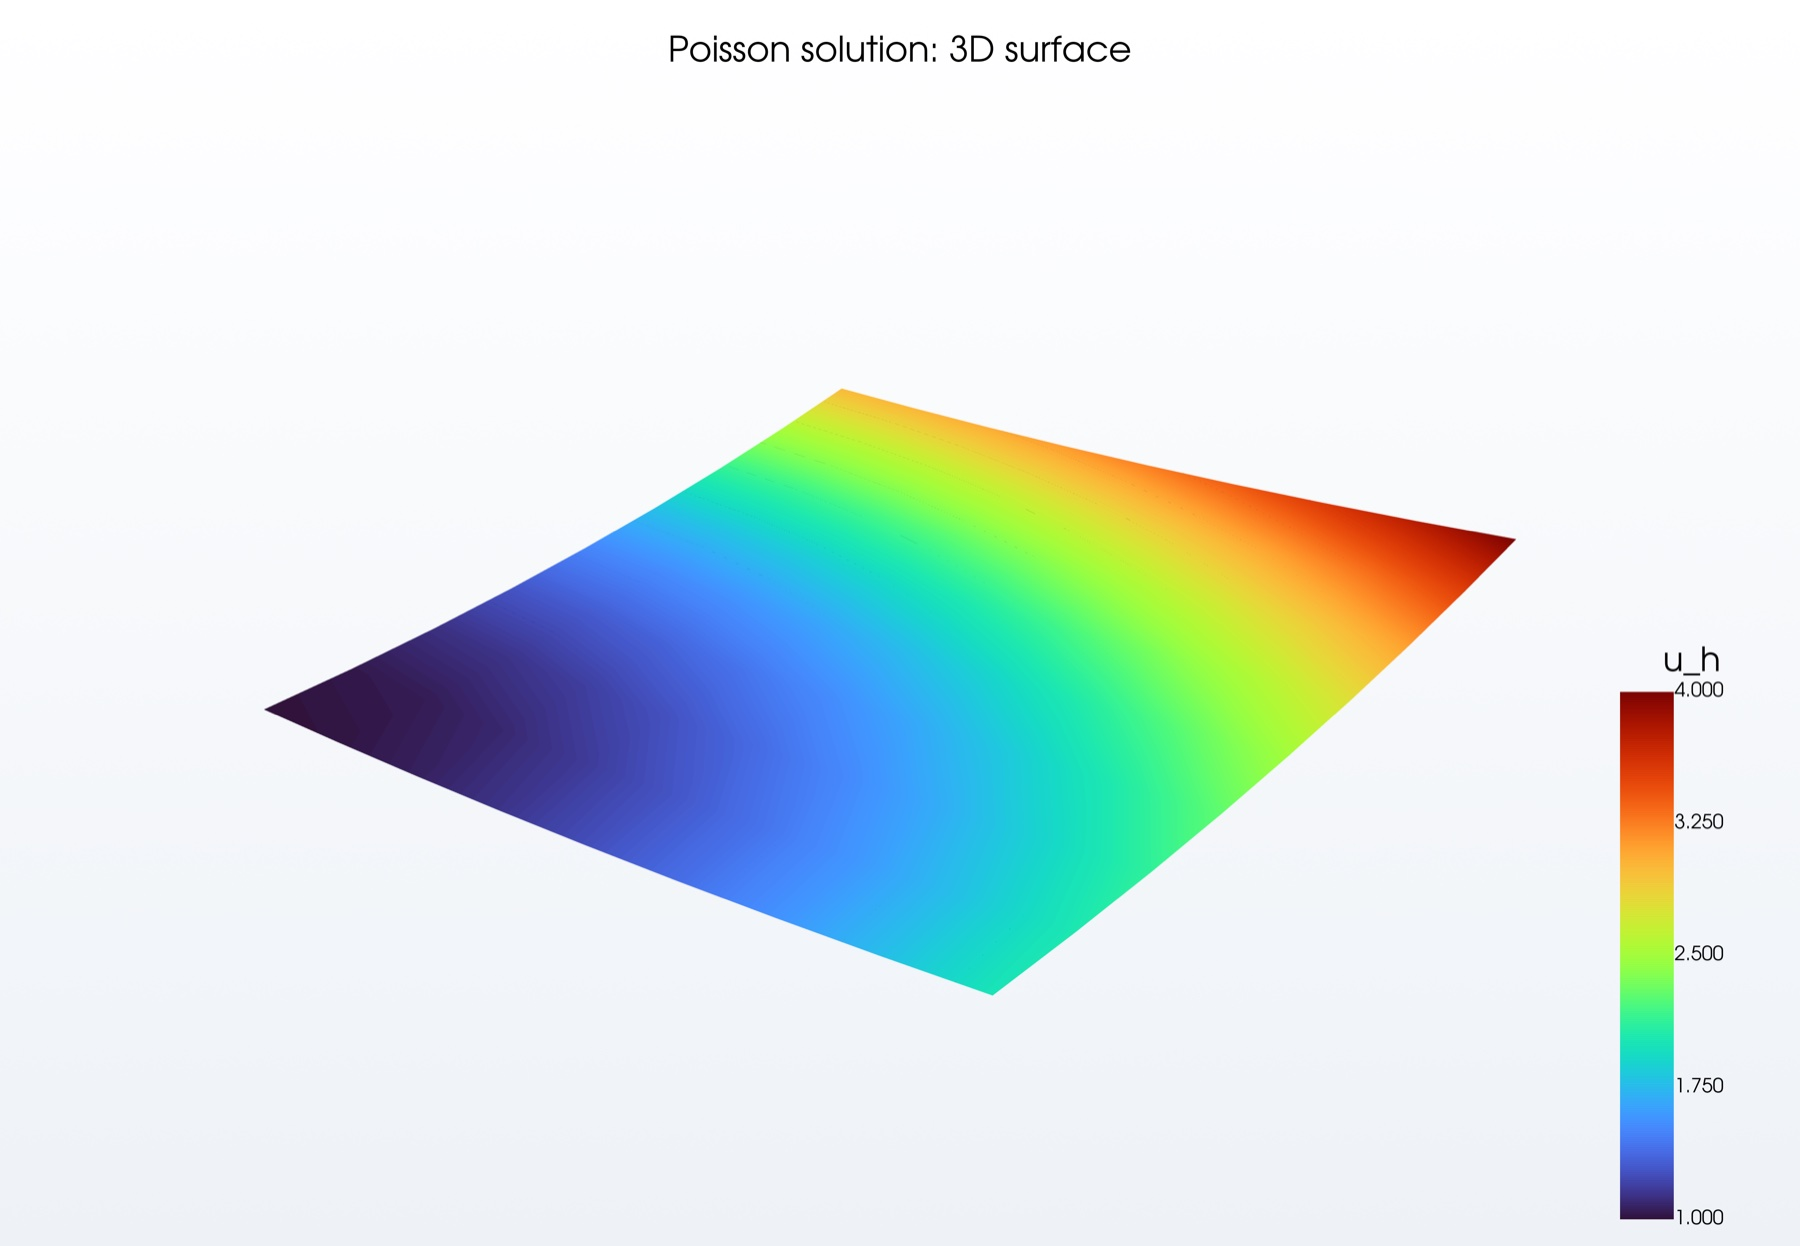
\includegraphics[width=0.495\textwidth]{poisson_solution_3d_slide.jpg}
\end{center}

\medskip
\small
The computed Poisson solution shown as a colour map and a surface.

\end{frame}

% ──────────────────────────────────────────────────────────────
\begin{frame}{Convergence study}

\begin{columns}[T]
\column{0.22\textwidth}

\tiny
Solve on meshes $N = 4, 8, 16, 32, 64, 128$.

\vspace{0.2em}
\setlength{\tabcolsep}{2.2pt}
\renewcommand{\arraystretch}{1.05}
\begin{tabular}{@{}cccc@{}}
\toprule
$N$ & $h$ & $\|e\|_{L^2}$ & $\|e\|_{H^1}$ \\
\midrule
4   & 0.354 & 5.27e-02 & 6.01e-01 \\
8   & 0.177 & 1.33e-02 & 3.02e-01 \\
16  & 0.088 & 3.33e-03 & 1.51e-01 \\
32  & 0.044 & 8.33e-04 & 7.56e-02 \\
64  & 0.022 & 2.08e-04 & 3.78e-02 \\
128 & 0.011 & 5.21e-05 & 1.89e-02 \\
\bottomrule
\end{tabular}

\column{0.76\textwidth}

\begin{center}
    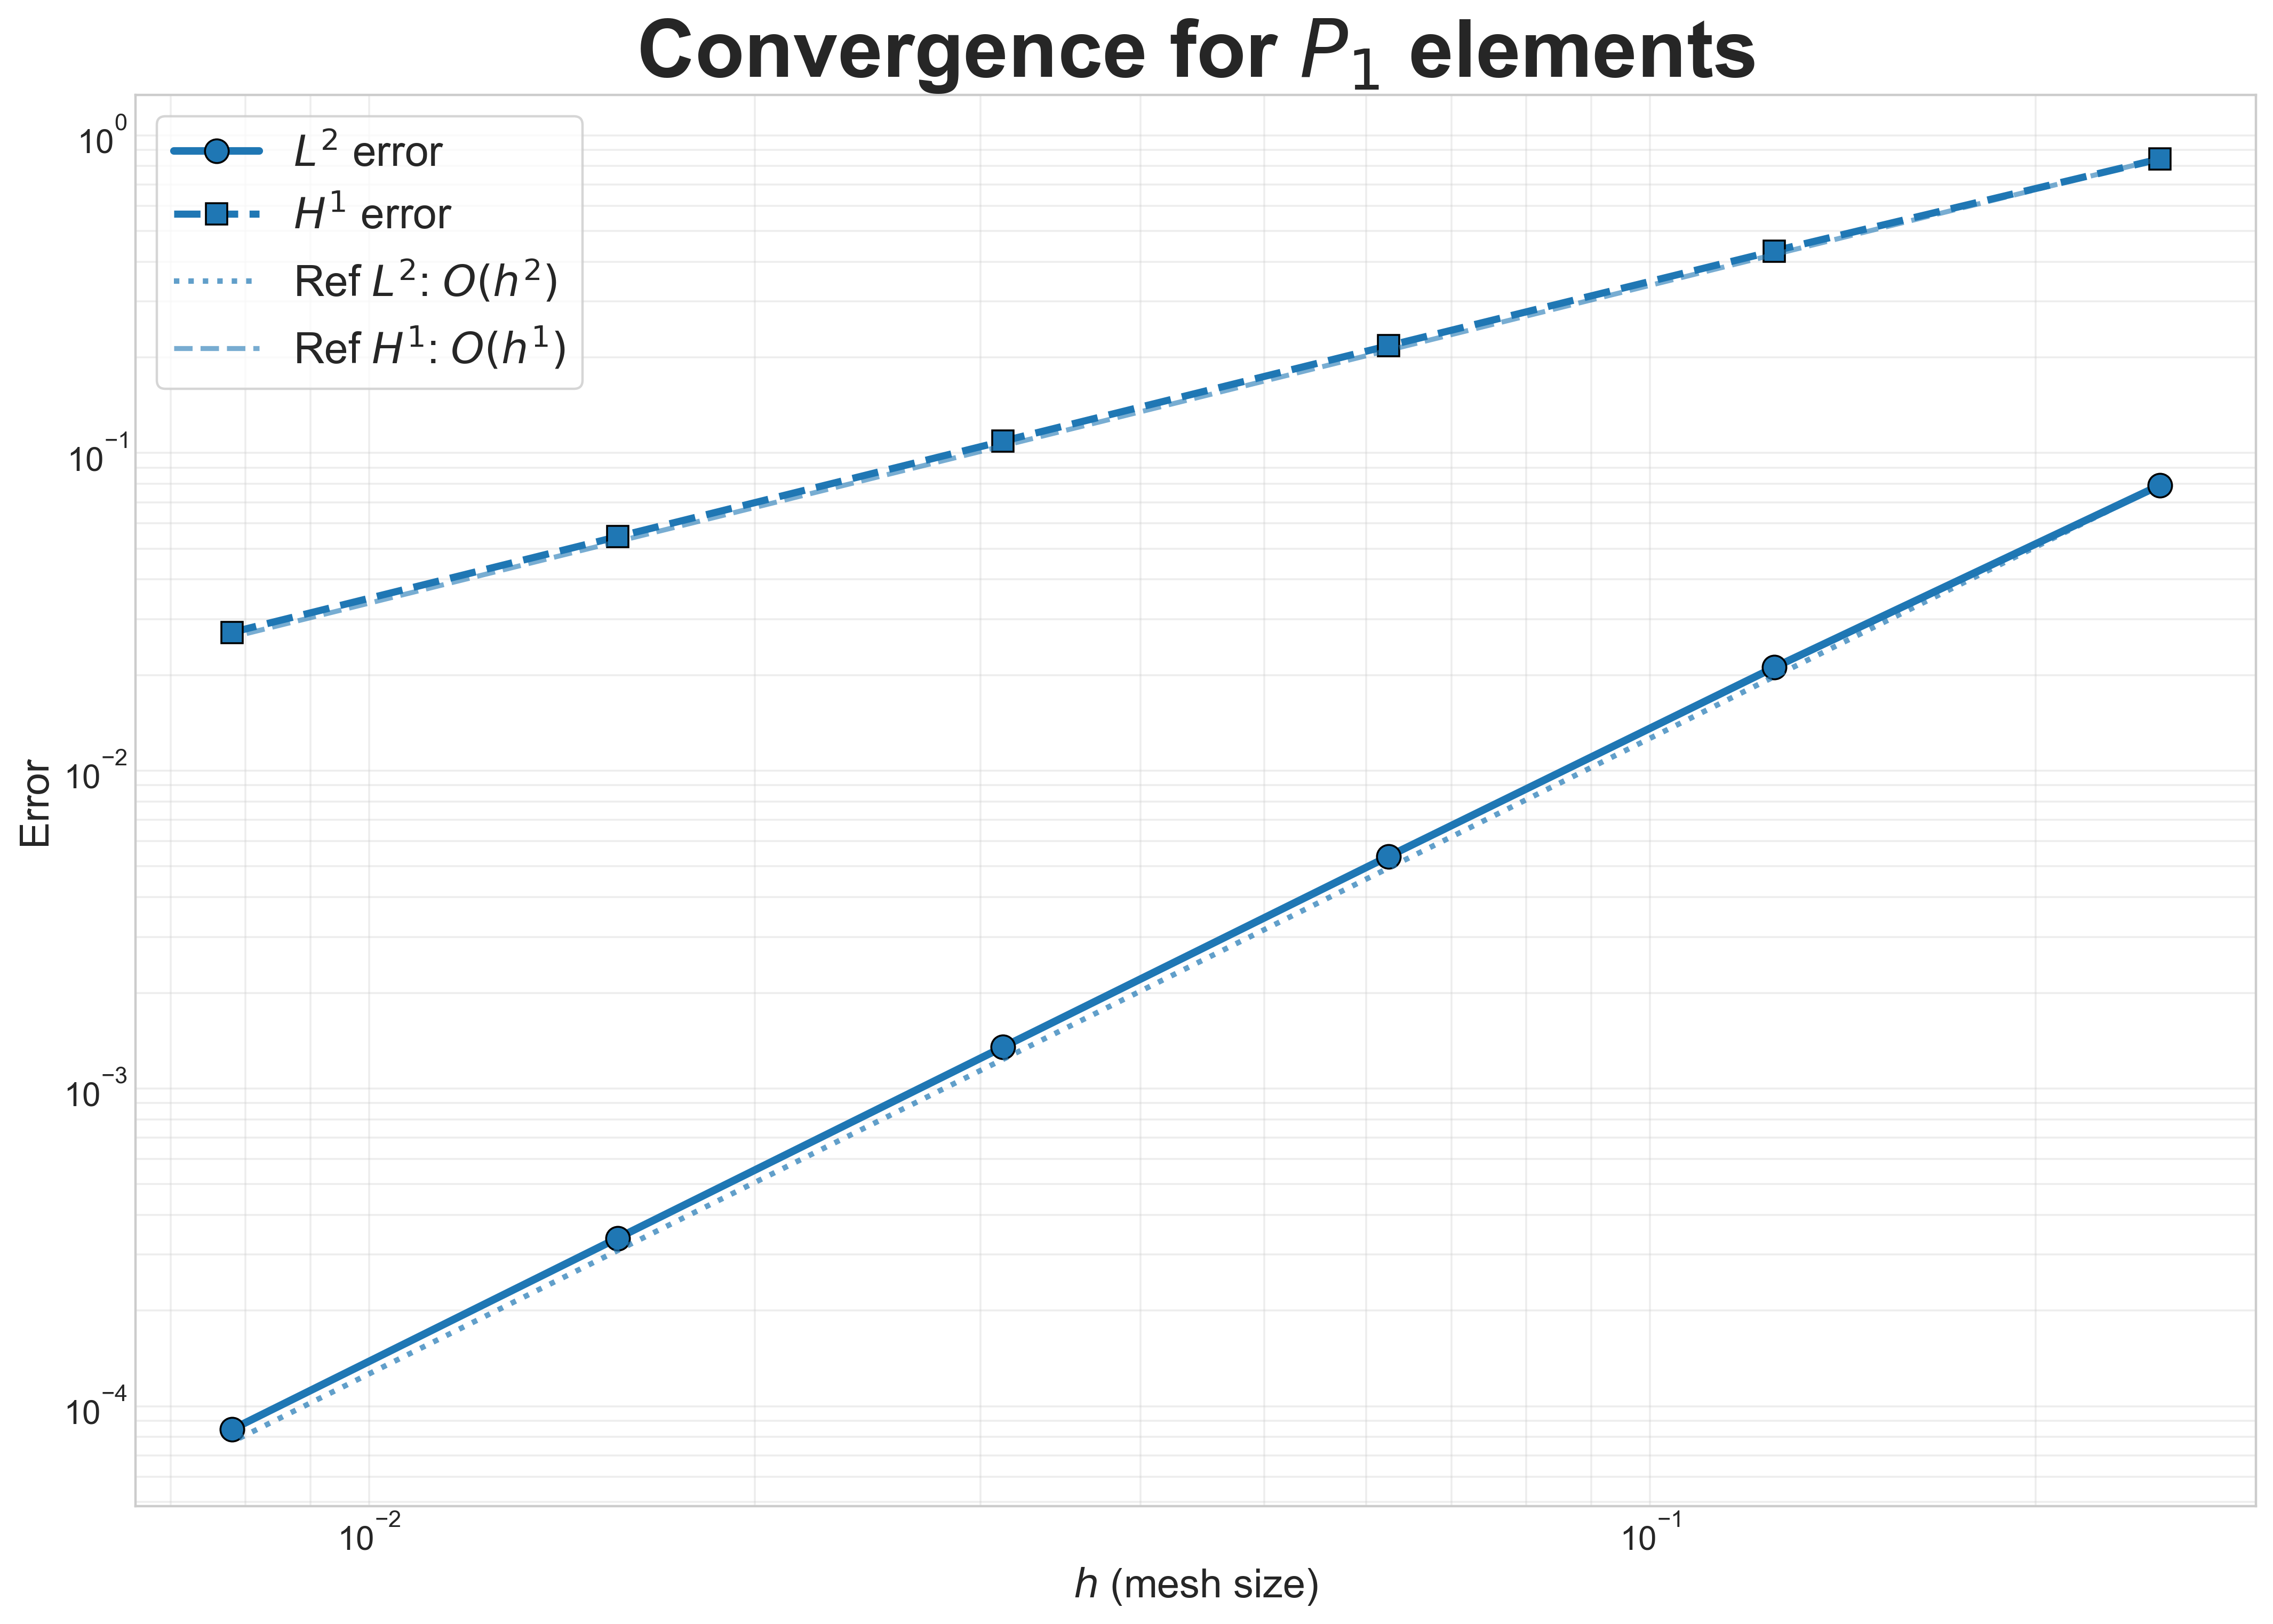
\includegraphics[width=0.49\linewidth]{convergence_plot_p1.png}
    \hfill
    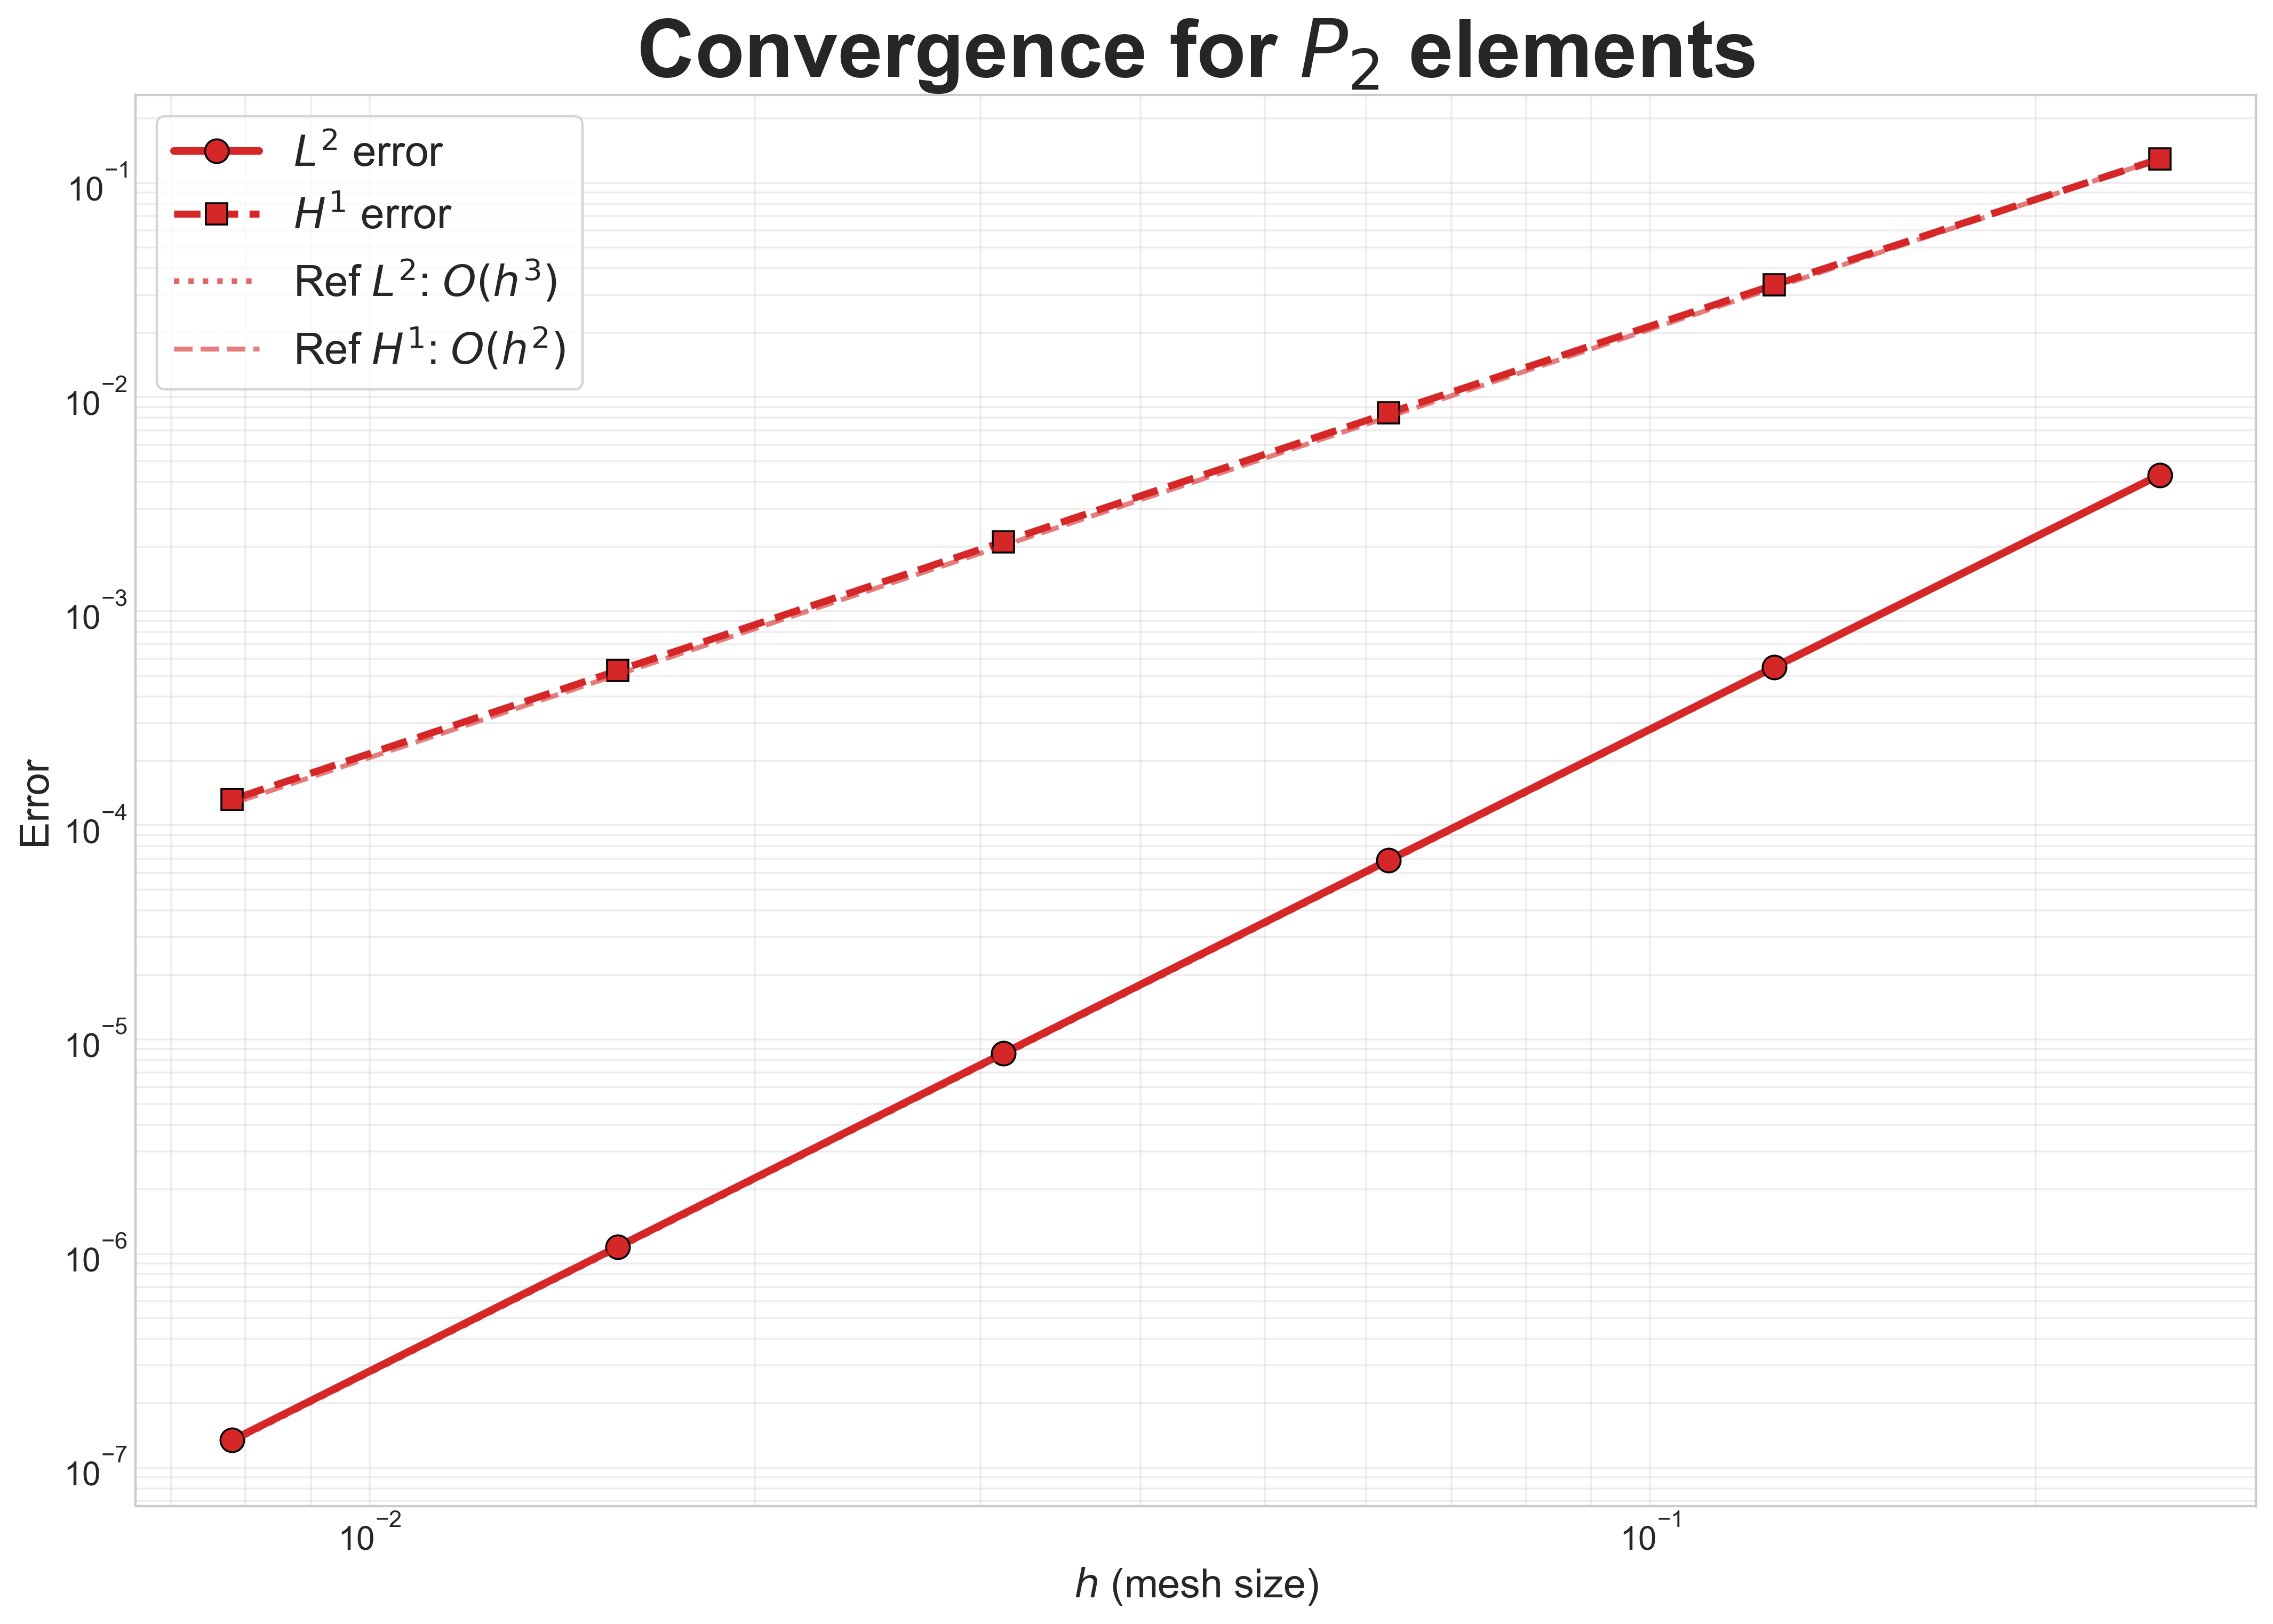
\includegraphics[width=0.49\linewidth]{convergence_plot_p2.png}
\end{center}

\end{columns}

\vspace{0.2em}
\footnotesize
$P_k$ elements: $\|u - u_h\|_{L^2} = O(h^{k+1})$, \;
$\|u - u_h\|_{H^1} = O(h^{k})$.\\
These convergence plots (left: $P_1$, right: $P_2$) confirm the expected rates.

\end{frame}

% ──────────────────────────────────────────────────────────────
\dividerframe{EXAMPLE 2}{Neumann problem with local mesh refinement}

% ──────────────────────────────────────────────────────────────
\begin{frame}{Elliptic example: Neumann BC + local refinement}

\begin{itemize}
\footnotesize
\item PDE on an L-shaped domain:
      $-\Delta u + u = f$ in $\Omega$, with homogeneous Neumann BC
      $\partial_n u = 0$ on $\partial\Omega$.
\item Explicit forcing:
    $f(x,y)=\dfrac{1}{\left(x^2+y^2+\varepsilon^2\right)^{3/4}}$, with
    $\varepsilon=6\times10^{-3}$.
\item This forcing is singular near the re-entrant corner,
      so local mesh refinement near $(0,0)$ gives better accuracy per DOF.
\item The script compares uniform refinement with refinement near the corner.
\end{itemize}

\medskip
\footnotesize
\textbf{Weak formulation} ($V = H^1(\Omega)$): find $u \in V$ such that
\[
\int_{\Omega} \nabla u \cdot \nabla v\,dx + \int_{\Omega} u\,v\,dx
= \int_{\Omega} f\,v\,dx
\quad \forall v \in V.
\]

\end{frame}

% ──────────────────────────────────────────────────────────────
\begin{frame}[fragile]{Neumann example: key code}

\begin{lstlisting}[basicstyle=\ttfamily\tiny]
V = fem.functionspace(msh, ("Lagrange", 1))
u = ufl.TrialFunction(V); v = ufl.TestFunction(V)
x = ufl.SpatialCoordinate(msh)
r2 = x[0]*x[0] + x[1]*x[1] + eps*eps
f_expr = 1.0 / (r2**0.75)

# Pure Neumann: no Dirichlet constraints
a = (ufl.inner(ufl.grad(u), ufl.grad(v)) + u*v) * ufl.dx
L = f_expr * v * ufl.dx
u_h = LinearProblem(a, L, bcs=[]).solve()

# Corner-focused weighted error metric
weight = ufl.exp(-(x[0]*x[0] + x[1]*x[1]) / (0.06**2))
E_corner = fem.assemble_scalar(fem.form(weight * u_h * ufl.dx))
\end{lstlisting}

\medskip
\begin{itemize}
\small
\item The extra $+u$ term makes the pure-Neumann model uniquely solvable.
\item Neumann data is natural in the weak form, so no boundary DOF constraints are added.
\item A weighted corner error metric near $(0,0)$ quantifies refinement accuracy.
\end{itemize}

\end{frame}

% ──────────────────────────────────────────────────────────────
\begin{frame}[fragile]{Adaptive mesh refinement (Neumann example)}

\begin{columns}[T]
\column{0.5\textwidth}

\begin{lstlisting}[basicstyle=\ttfamily\tiny]
# Error indicator
e = u_exact - u_h
indicators = project(
    inner(grad(e), grad(e)), DG0)

# Mark cells with large error
cell_markers = MeshFunction(
    "bool", mesh,
    mesh.topology().dim(), False)

# Refine top 30% of cells
cutoff = sorted(indicators.vector()[:],
    reverse=True)[int(0.3*mesh.num_cells())]

for c in cells(mesh):
    if indicators(c.midpoint()) > cutoff:
        cell_markers[c] = True

mesh = refine(mesh, cell_markers)
\end{lstlisting}

\column{0.45\textwidth}

\begin{center}
    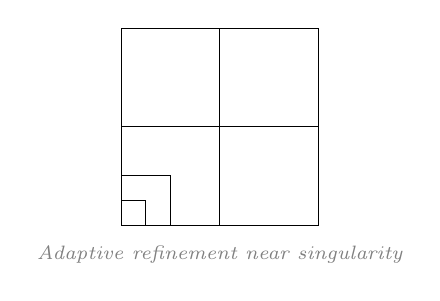
\begin{tikzpicture}[scale=2.5]
    % Coarse mesh suggestion
    \draw[thin] (0,0) rectangle (1,1);
    \draw[thin] (0.5,0) -- (0.5,1);
    \draw[thin] (0,0.5) -- (1,0.5);
    % Refined corner
    \draw[thin] (0,0) -- (0.25,0) -- (0.25,0.25) -- (0,0.25) -- cycle;
    \draw[thin] (0.25,0) -- (0.5,0);
    \draw[thin] (0,0.25) -- (0,0.5);
    \draw[thin] (0.125,0) -- (0.125,0.125);
    \draw[thin] (0,0.125) -- (0.125,0.125);
    \node[font=\scriptsize\itshape, text=gray] at (0.5, -0.15)
        {Adaptive refinement near singularity};
    \end{tikzpicture}
\end{center}

\end{columns}

\end{frame}

% ──────────────────────────────────────────────────────────────
\begin{frame}{Neumann example: results}

\begin{center}
    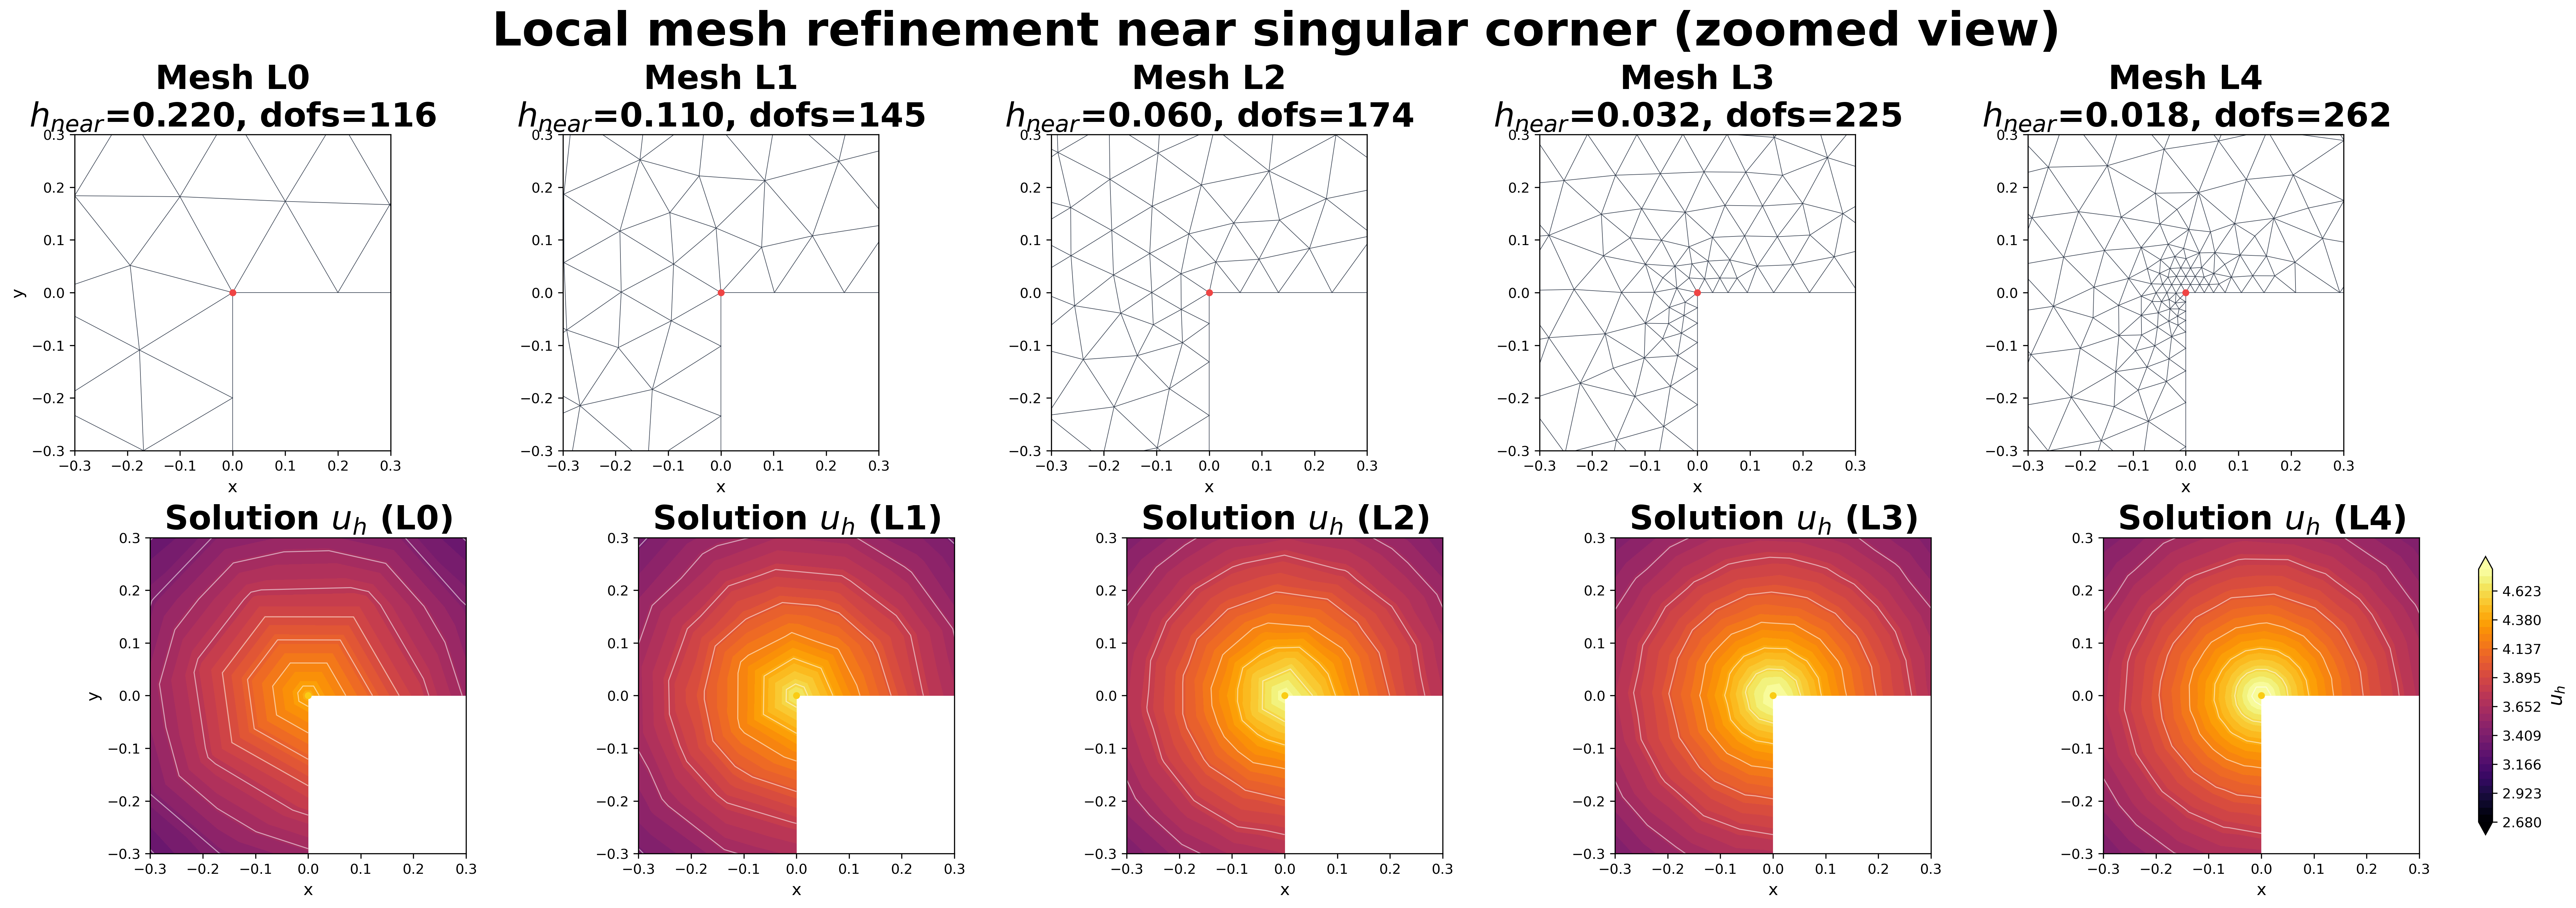
\includegraphics[width=0.67\textwidth]{neumann_refinement.png}
    \hfill
    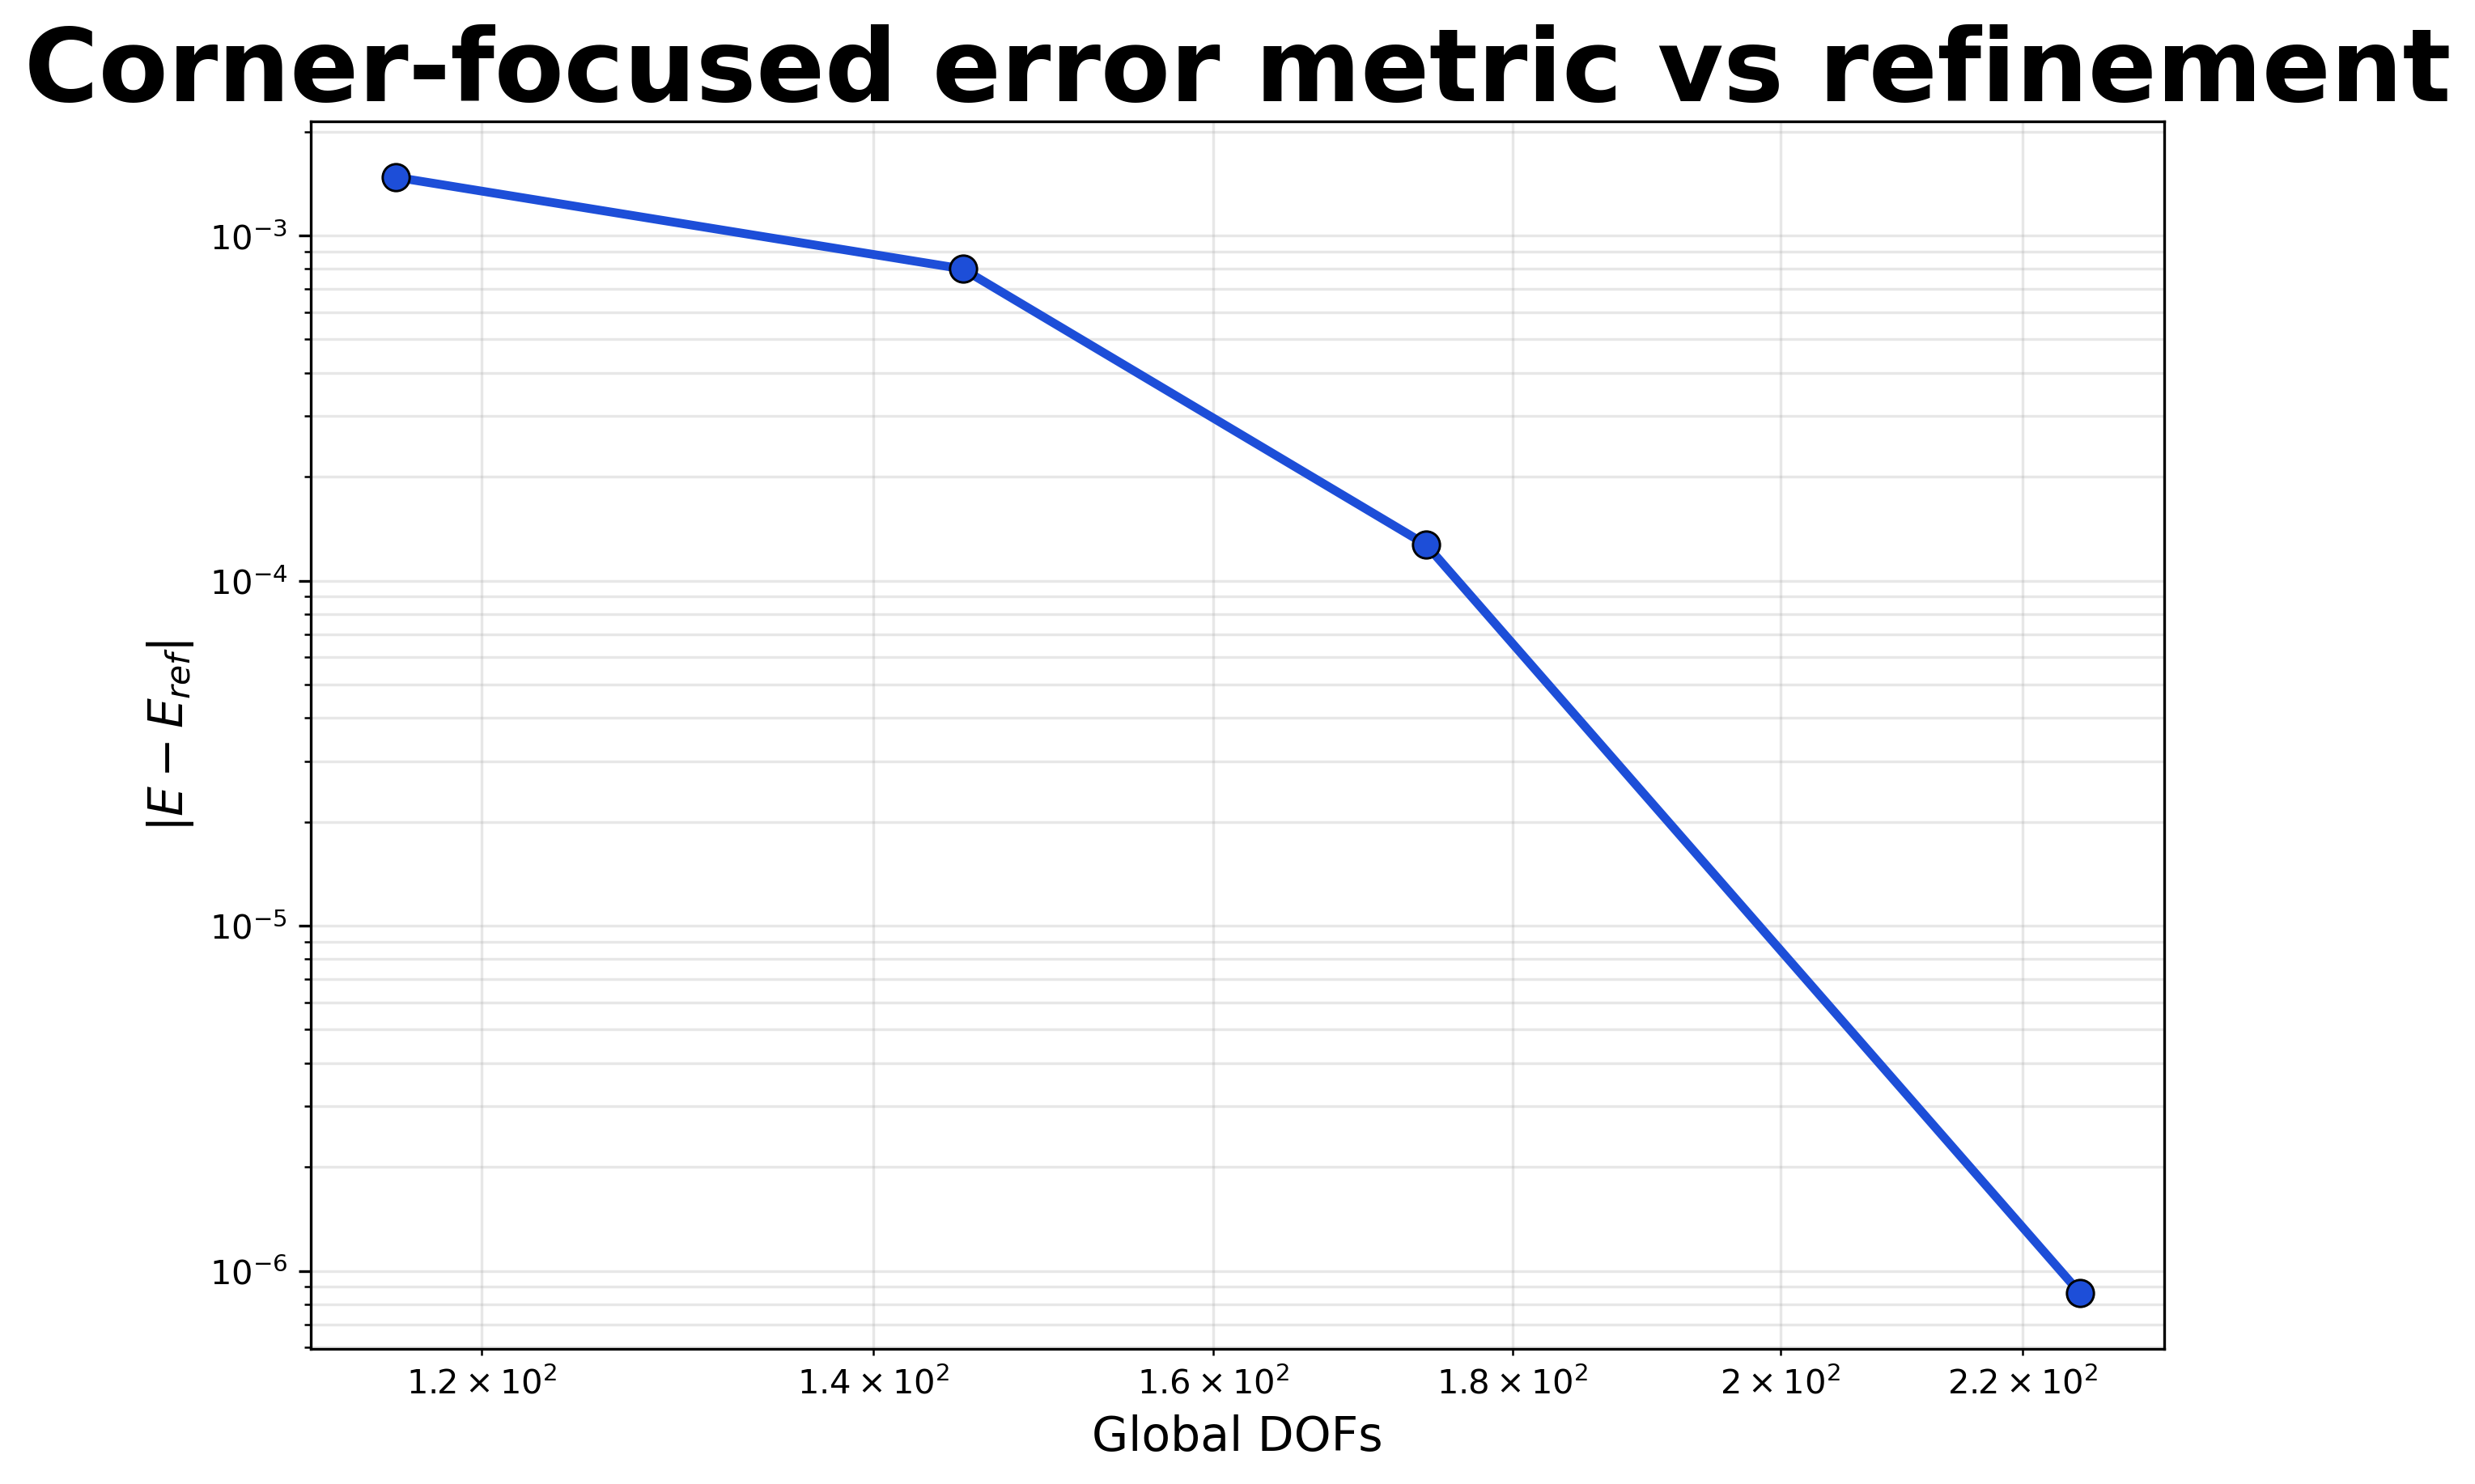
\includegraphics[width=0.31\textwidth]{neumann_refinement_error_metric.png}
\end{center}

\medskip
\small
Local refinement near the re-entrant corner improves both field resolution and
the corner-weighted error-metric convergence.

\end{frame}

% ──────────────────────────────────────────────────────────────
\dividerframe{EXAMPLE 3}{L-shaped Laplacian eigenfunction}

% ──────────────────────────────────────────────────────────────
\begin{frame}{Elliptic example: L-shaped Laplacian eigenfunction}

\begin{itemize}
\footnotesize
\item Eigenproblem on an L-shaped domain:
      $-\Delta \phi = \lambda\,\phi$ in $\Omega$, with $\phi=0$ on $\partial\Omega$.
\item The re-entrant corner induces singular behavior and a characteristic mode shape.
\item Compute the first eigenmode and inspect its behaviour near the corner.
\end{itemize}

\medskip
\footnotesize
\textbf{Weak formulation} ($V = H_0^1(\Omega)$): find $(\lambda, \phi) \in \mathbb{R} \times V$, $\phi \neq 0$, such that
\[
\int_{\Omega} \nabla \phi \cdot \nabla v\,dx
= \lambda \int_{\Omega} \phi\,v\,dx
\quad \forall v \in V.
\]

\vspace{-0.3em}
\footnotesize
\textit{Handling $(\lambda,\phi)\in\mathbb{R}\times V$:} discretize only $\phi$ in $V_h$,
obtain $A\Phi = \lambda M\Phi$, and fix the scale with
$\Phi^T M\Phi=1$ (equivalently $\|\phi_h\|_{L^2(\Omega)}=1$).

\end{frame}

% ──────────────────────────────────────────────────────────────
\begin{frame}[fragile]{L-shaped eigenproblem: key code}

\begin{lstlisting}[basicstyle=\ttfamily\tiny]
u = ufl.TrialFunction(V); v = ufl.TestFunction(V)
A = assemble_matrix(fem.form(inner(grad(u), grad(v))*dx)); A.assemble()
M = assemble_matrix(fem.form(u*v*dx)); M.assemble()
A_sp = petsc_to_scipy(A); M_sp = petsc_to_scipy(M)

# Enforce phi=0 on boundary by removing boundary dofs
free_dofs = np.setdiff1d(np.arange(num_dofs), boundary_dofs)
A_free = A_sp[free_dofs][:, free_dofs]
M_free = M_sp[free_dofs][:, free_dofs]

eigvals, eigvecs = eigsh(A_free, k=8, M=M_free, sigma=0.0, which="LM")
phi = np.zeros(num_dofs)
phi[free_dofs] = eigvecs[:, 0]
phi /= np.max(np.abs(phi))
\end{lstlisting}

\medskip
\begin{itemize}
\small
\item This solves the generalized eigenproblem $A\phi = \lambda M\phi$.
\item Boundary elimination strongly enforces homogeneous Dirichlet conditions.
\item Plot the normalized first mode as contours and as a surface.
\end{itemize}

\end{frame}

% ──────────────────────────────────────────────────────────────
\begin{frame}{L-shaped eigenproblem: results}

\begin{center}
    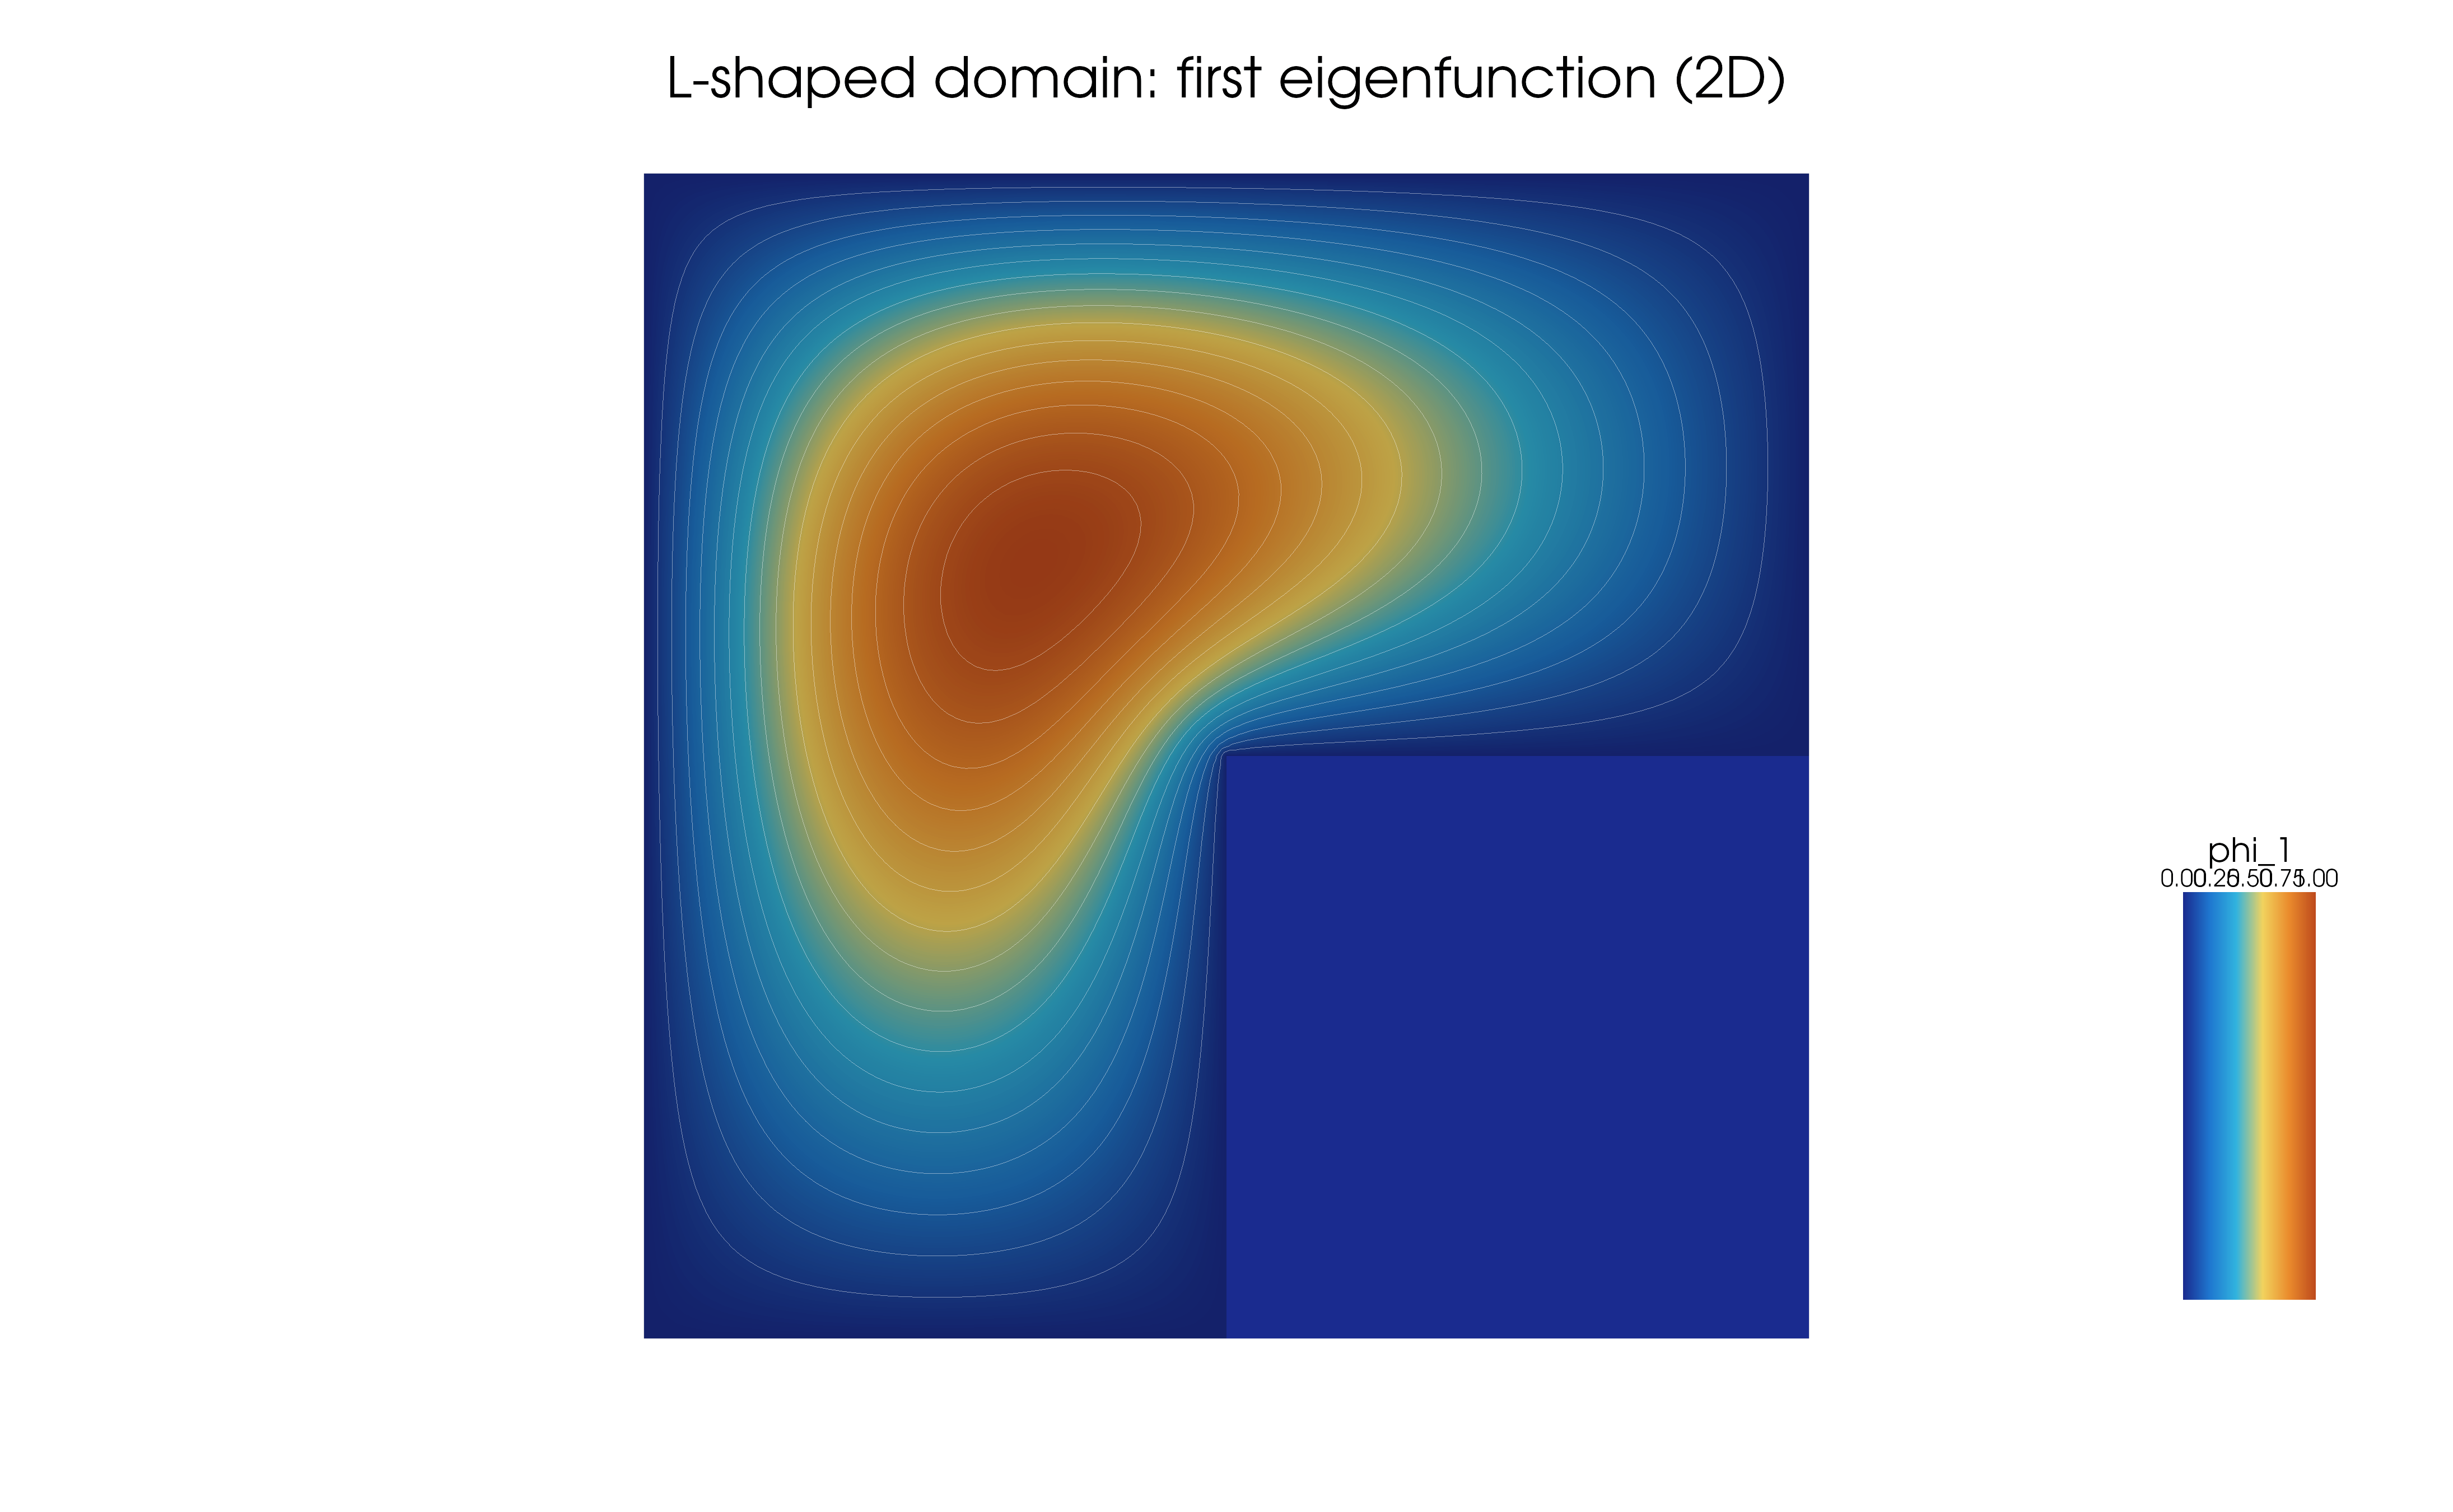
\includegraphics[width=0.48\textwidth]{lshape_eigenfunction_2d.png}
    \hfill
    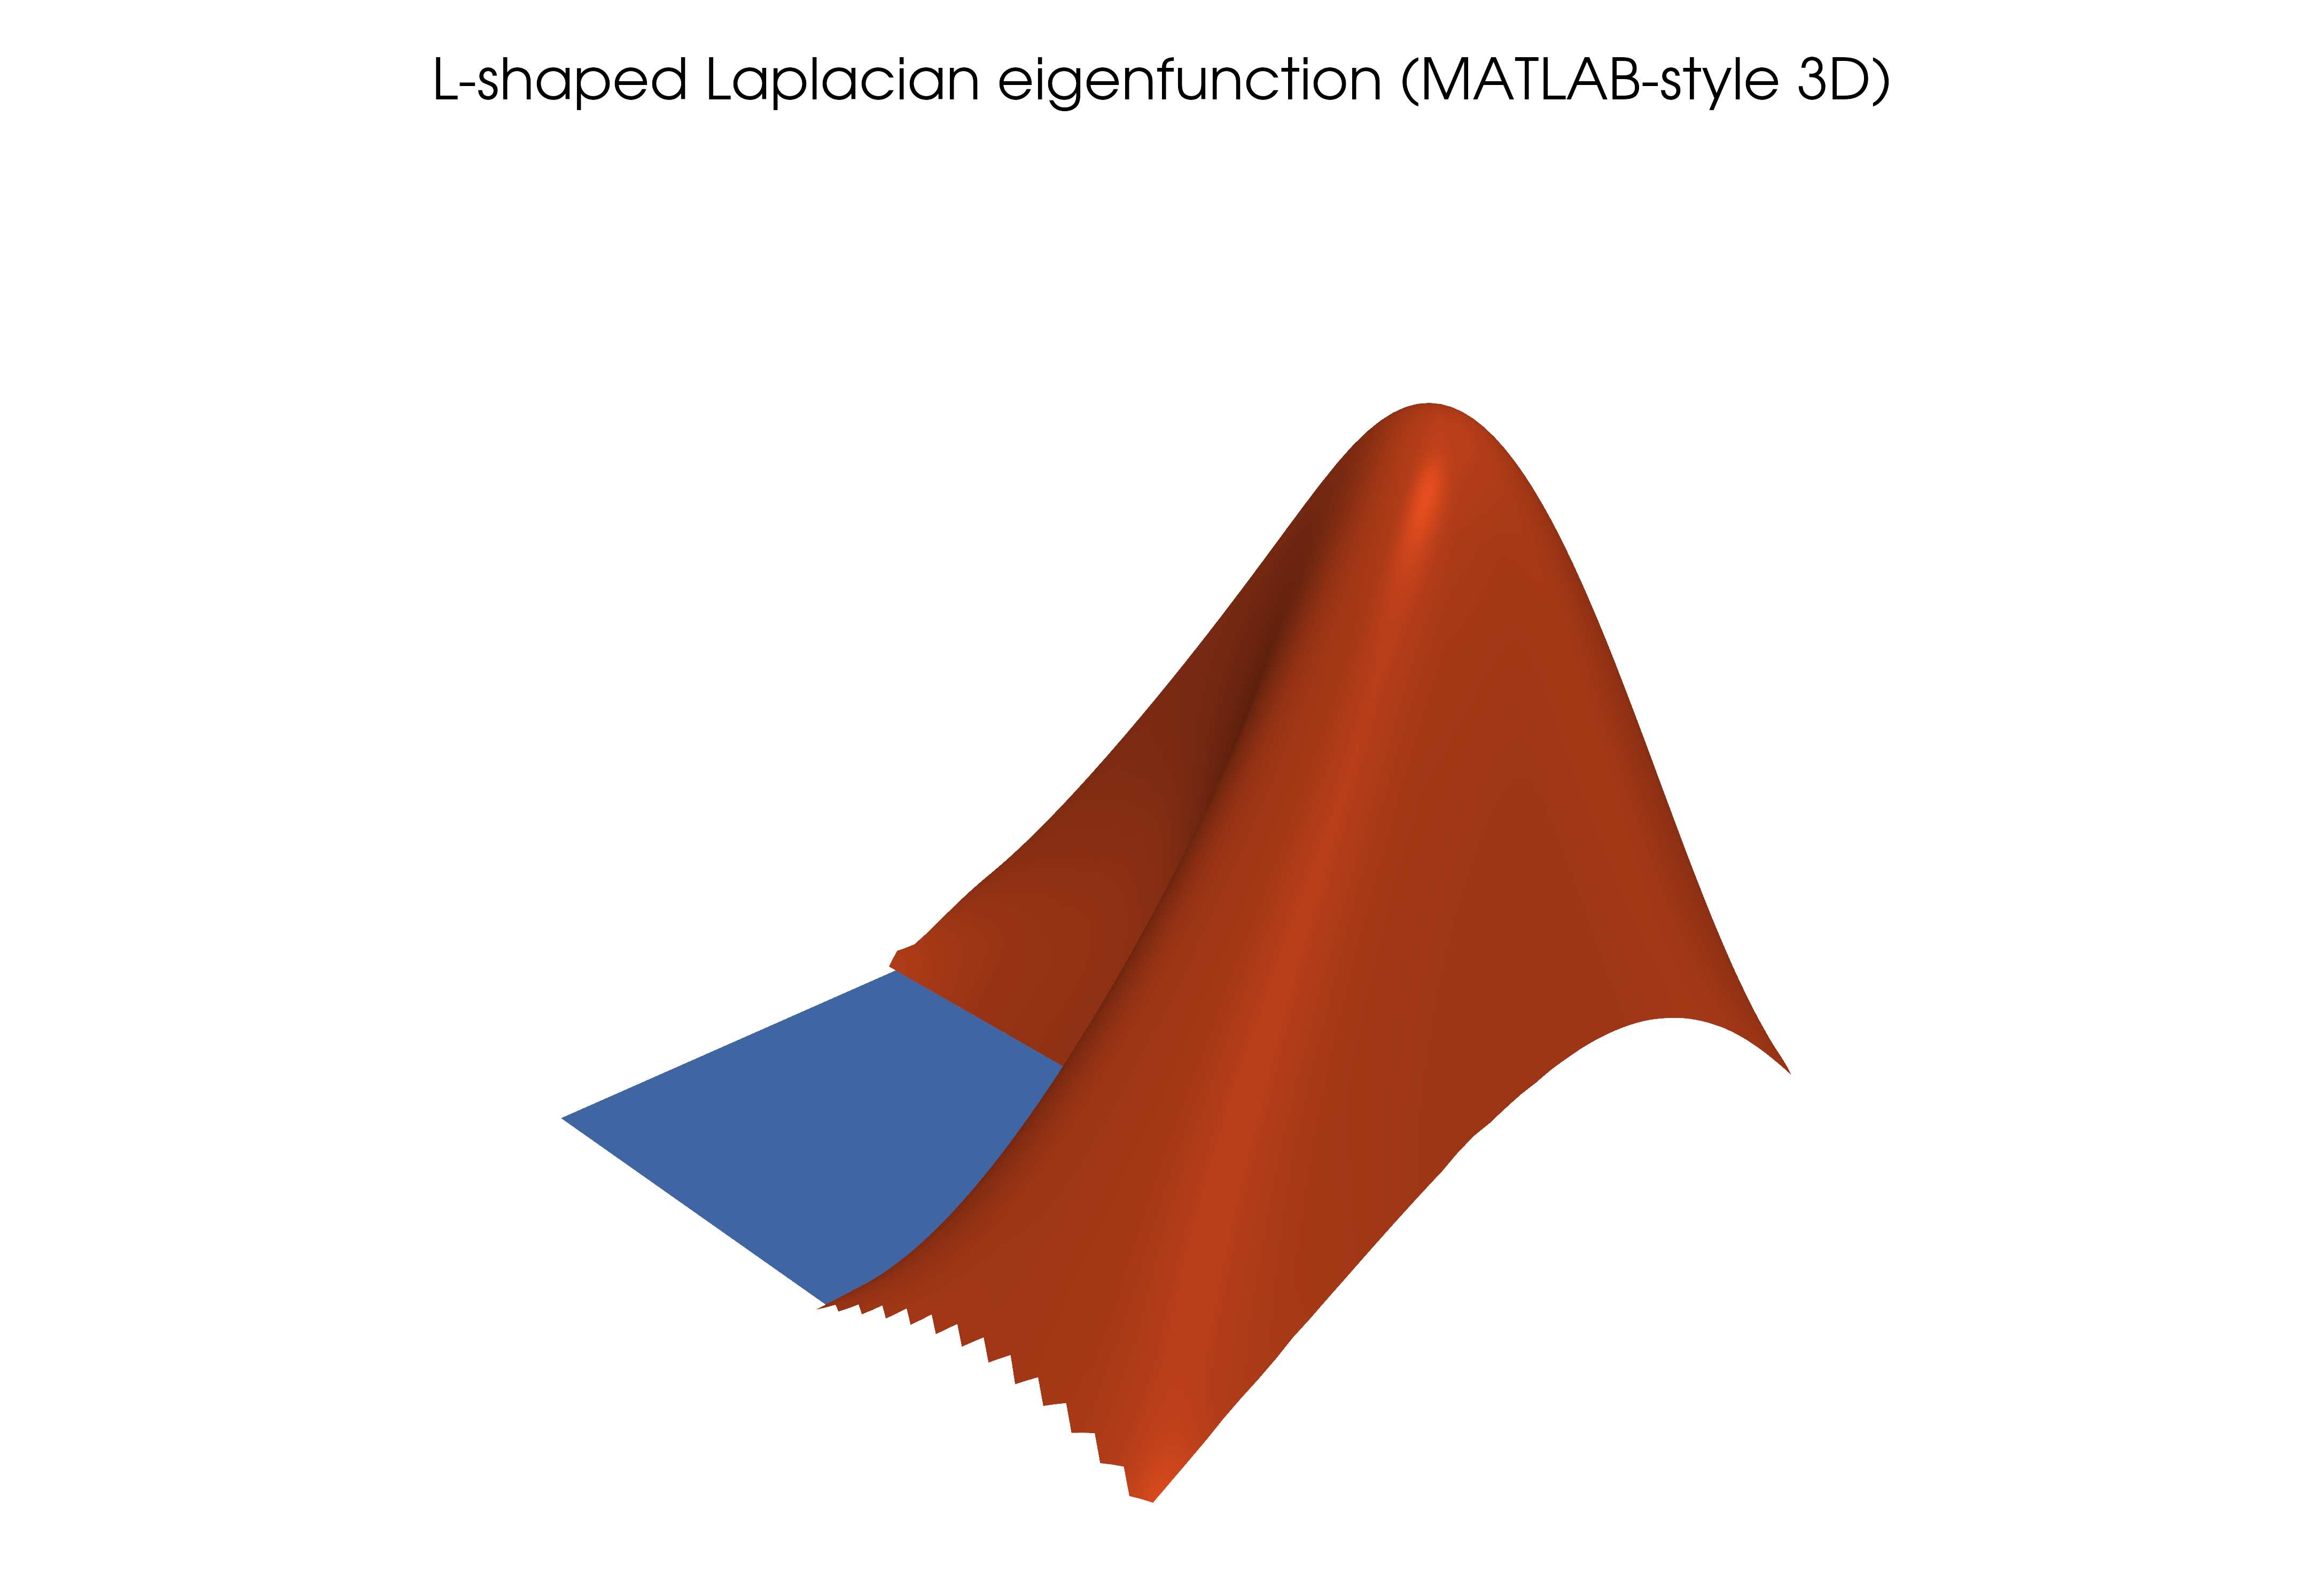
\includegraphics[width=0.48\textwidth]{lshape_eigenfunction_3d_matlab.png}
\end{center}

\end{frame}

% ══════════════════════════════════════════════════════════════
\section{Time-dependent problems}
% ══════════════════════════════════════════════════════════════

% ──────────────────────────────────────────────────────────────
\dividerframe{EXAMPLE 4}{Heat equation}

% ──────────────────────────────────────────────────────────────
\begin{frame}{Heat equation}

\begin{block}{Problem}
\[
    \frac{\partial u}{\partial t} - \Delta u = 0 \quad \text{in } \Omega \times (0, T]
\]
$u = 0$ on $\partial\Omega$, \quad
$u(x, 0) = \exp\bigl(-25\,\|(x - \tfrac{1}{2}, y-\tfrac{1}{2})\|^2\bigr)$
\end{block}

\medskip

\textbf{Backward Euler} time discretization:
\[
    \frac{u^{n+1} - u^n}{\Delta t} - \Delta u^{n+1} = 0
\]

Weak form at each step:
\[
  \underbrace{(u^{n+1}, v) + \Delta t\,(\nabla u^{n+1}, \nabla v)}_{a(u^{n+1}, v)}
  = \underbrace{(u^n, v)}_{L(v)}
\]

\end{frame}

% ──────────────────────────────────────────────────────────────
\begin{frame}[fragile]{Heat equation: code}

\begin{lstlisting}[basicstyle=\ttfamily\tiny]
dt = T / num_steps
mesh = UnitSquareMesh(30, 30)
V = FunctionSpace(mesh, 'P', 1)
bc = DirichletBC(V, Constant(0.0), 'on_boundary')

# Initial condition: Gaussian bump
u_n = interpolate(Expression(
    'exp(-25*((x[0]-0.5)*(x[0]-0.5)+(x[1]-0.5)*(x[1]-0.5)))',
    degree=2), V)

u = TrialFunction(V);  v = TestFunction(V)

# Backward Euler weak form
a = u*v*dx + dt*dot(grad(u), grad(v))*dx
L = u_n*v*dx

u_h = Function(V)
for n in range(num_steps):
    solve(a == L, u_h, bc)    # Solve one time step
    u_n.assign(u_h)           # Update u^n <- u^{n+1}
\end{lstlisting}

\medskip

\textbf{Reuse the matrix:} With constant $\Delta t$, the bilinear form
\texttt{a} stays the same. A solver configured to reuse its factorization
can avoid repeating that work.

\end{frame}

% ──────────────────────────────────────────────────────────────
\begin{frame}{Heat equation: solution snapshots}

\begin{center}
    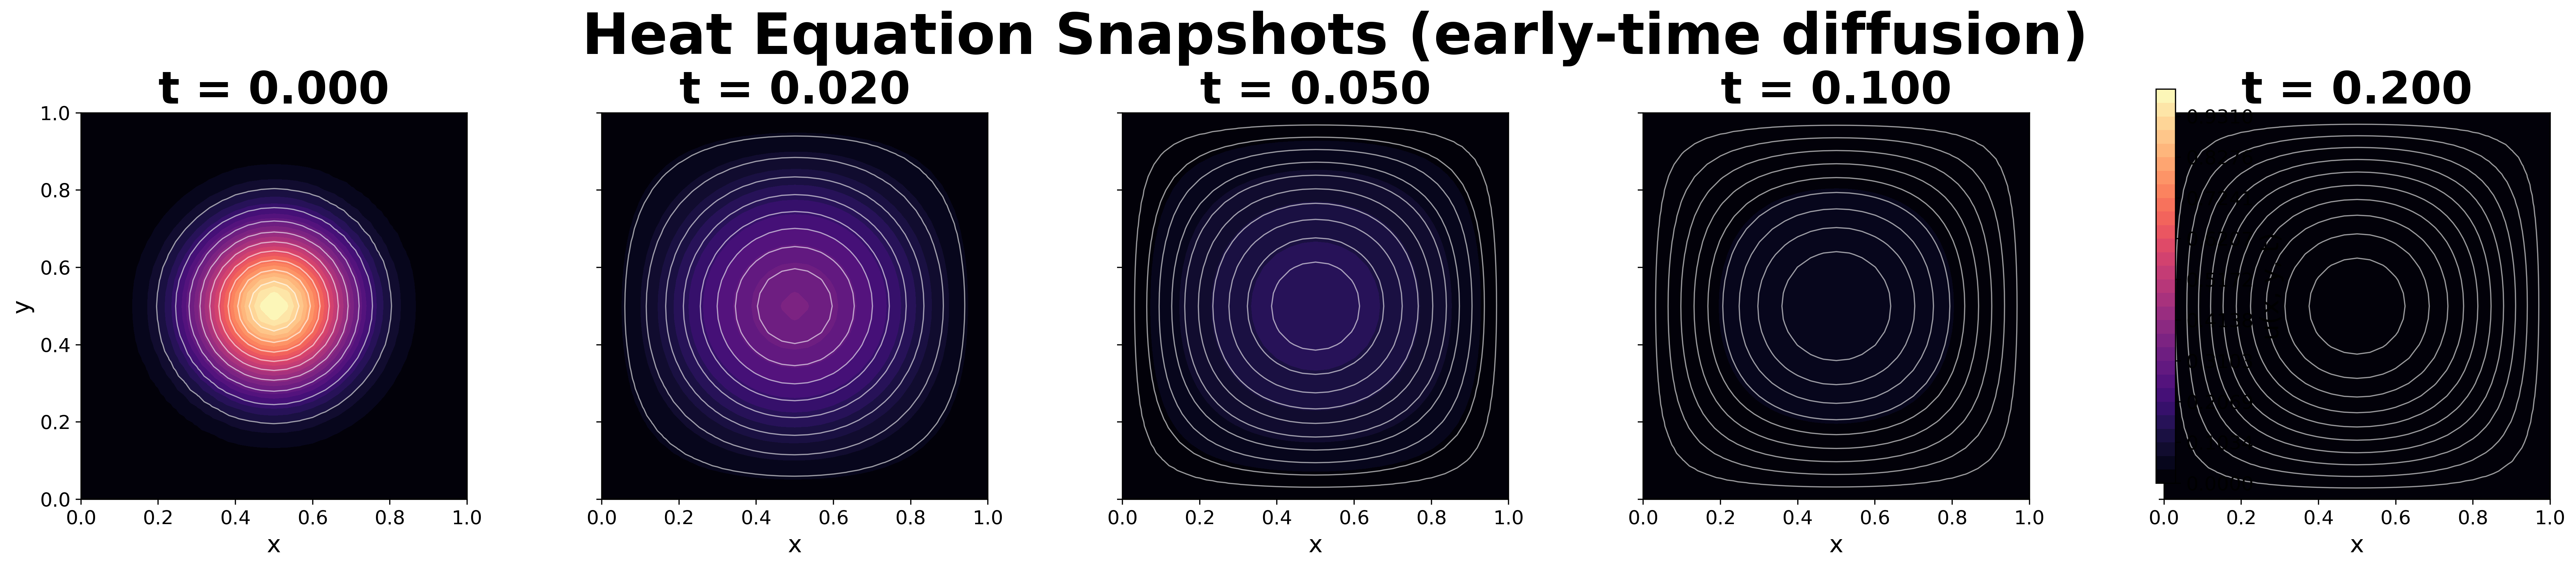
\includegraphics[width=\textwidth]{heat_equation.png}
\end{center}

\medskip
The Gaussian bump spreads and decreases in height as heat diffuses.

\end{frame}

% ══════════════════════════════════════════════════════════════
\section{Nonlinear problems}
% ══════════════════════════════════════════════════════════════

% ──────────────────────────────────────────────────────────────
\dividerframe{EXAMPLE 5}{Nonlinear Poisson equation}

% ──────────────────────────────────────────────────────────────
\begin{frame}{Nonlinear Poisson equation}

\begin{block}{Problem}
\[
  -\nabla \cdot \bigl( (1 + u^2)\, \nabla u \bigr) = f \quad \text{in } \Omega,
  \qquad u = 0 \text{ on } \partial\Omega
\]
\end{block}

\medskip

This is a \textbf{quasilinear} PDE --- the diffusion coefficient depends on $u$.

\medskip

\textbf{Residual form:} Find $u \in V$ such that
\[
  F(u; v) = \int_\Omega (1 + u^2)\, \nabla u \cdot \nabla v \, dx
           - \int_\Omega f \, v \, dx = 0
  \quad \forall v \in \hat{V}
\]

\medskip
FEniCS solves this with \textbf{Newton's method}.\\
The Jacobian $J = F'(u)$ can be computed \emph{automatically}.

\end{frame}

% ──────────────────────────────────────────────────────────────
\begin{frame}[fragile]{Nonlinear Poisson: code}

\begin{lstlisting}
# u is a Function (NOT TrialFunction) for
# nonlinear problems
u = Function(V)
v = TestFunction(V)

# Residual F(u; v) = 0
F = (1 + u**2)*dot(grad(u), grad(v))*dx \
    - f*v*dx

# Automatic Jacobian
J = derivative(F, u)

# Newton solver
problem = NonlinearVariationalProblem(F, u, bc, J)
solver  = NonlinearVariationalSolver(problem)
solver.solve()
\end{lstlisting}

\bigskip
\small
\textbf{For a nonlinear problem:}
\texttt{TrialFunction} $\to$ \texttt{Function} (an unknown to be solved for iteratively).

\end{frame}

% ══════════════════════════════════════════════════════════════
\section{Mixed finite elements: Stokes equations}
% ══════════════════════════════════════════════════════════════

% ──────────────────────────────────────────────────────────────
\dividerframe{EXAMPLE 6}{Stokes flow in a lid-driven cavity}

% ──────────────────────────────────────────────────────────────
\begin{frame}{Stokes equations --- lid-driven cavity}

\begin{block}{Problem}
\begin{align*}
    -\Delta \mathbf{u} + \nabla p &= \mathbf{0} \quad &&\text{in } \Omega \\
  \nabla \cdot \mathbf{u} &= 0 \quad &&\text{in } \Omega \\
  \mathbf{u} &= (1,0) \quad &&\text{on top wall} \\
  \mathbf{u} &= \mathbf{0} \quad &&\text{on other walls}
\end{align*}
\end{block}

\medskip

\textbf{Mixed weak form:} Find $(\mathbf{u}, p) \in V \times Q$ such that
\begin{align*}
  (\nabla \mathbf{u}, \nabla \mathbf{v}) - (p, \nabla \cdot \mathbf{v})
  - (q, \nabla \cdot \mathbf{u}) &= 0
\end{align*}
for all $(\mathbf{v}, q) \in V \times Q$.

\medskip
\textbf{Inf-sup stability:} Use Taylor--Hood elements ($P_2/P_1$).

\end{frame}

% ──────────────────────────────────────────────────────────────
\begin{frame}[fragile]{Stokes: code}

\begin{lstlisting}[basicstyle=\ttfamily\tiny]
# Taylor-Hood: P2 velocity, P1 pressure
V = VectorFunctionSpace(mesh, 'P', 2)
Q = FunctionSpace(mesh, 'P', 1)
W = V * Q                               # Mixed space

# Boundary conditions
bc_lid   = DirichletBC(W.sub(0), Constant((1,0)),
                       'near(x[1],1.0) && on_boundary')
bc_walls = DirichletBC(W.sub(0), Constant((0,0)),
    '(near(x[0],0)||near(x[0],1)||near(x[1],0)) && on_boundary')

# Weak form
(u, p) = TrialFunctions(W)
(v, q) = TestFunctions(W)

a = (inner(grad(u), grad(v)) - p*div(v) - q*div(u)) * dx
L = inner(Constant((0, 0)), v) * dx

w = Function(W)
solve(a == L, w, [bc_lid, bc_walls])

(u_h, p_h) = w.split()  # Extract velocity and pressure
\end{lstlisting}

\end{frame}

% ──────────────────────────────────────────────────────────────
\begin{frame}{Stokes: results}

\begin{center}
    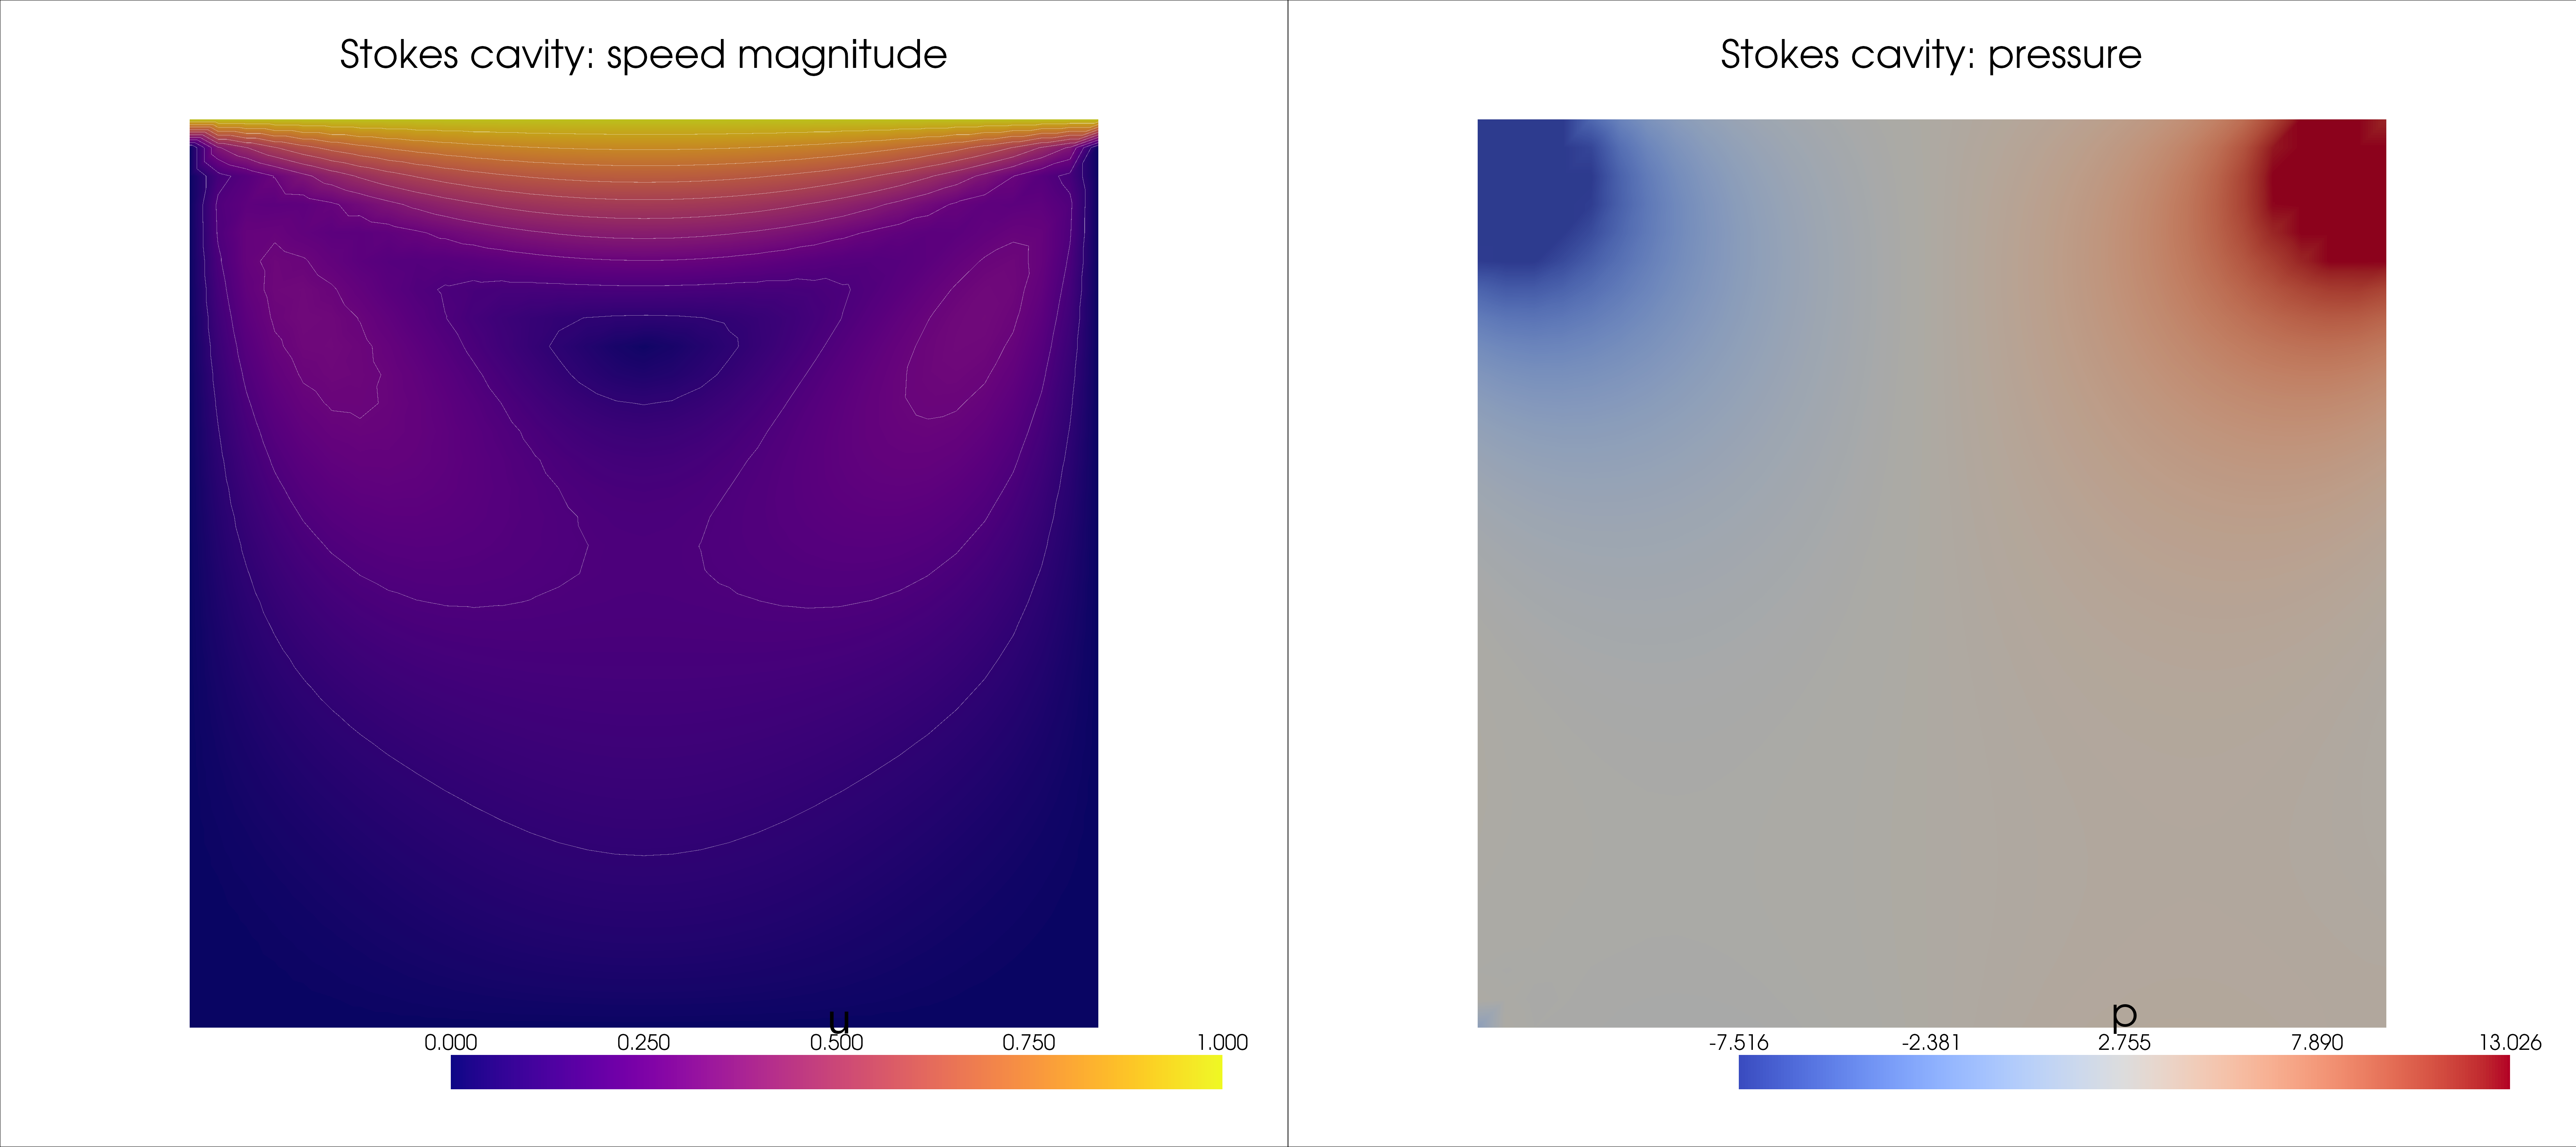
\includegraphics[width=0.495\textwidth]{stokes_cavity.png}
    \hfill
    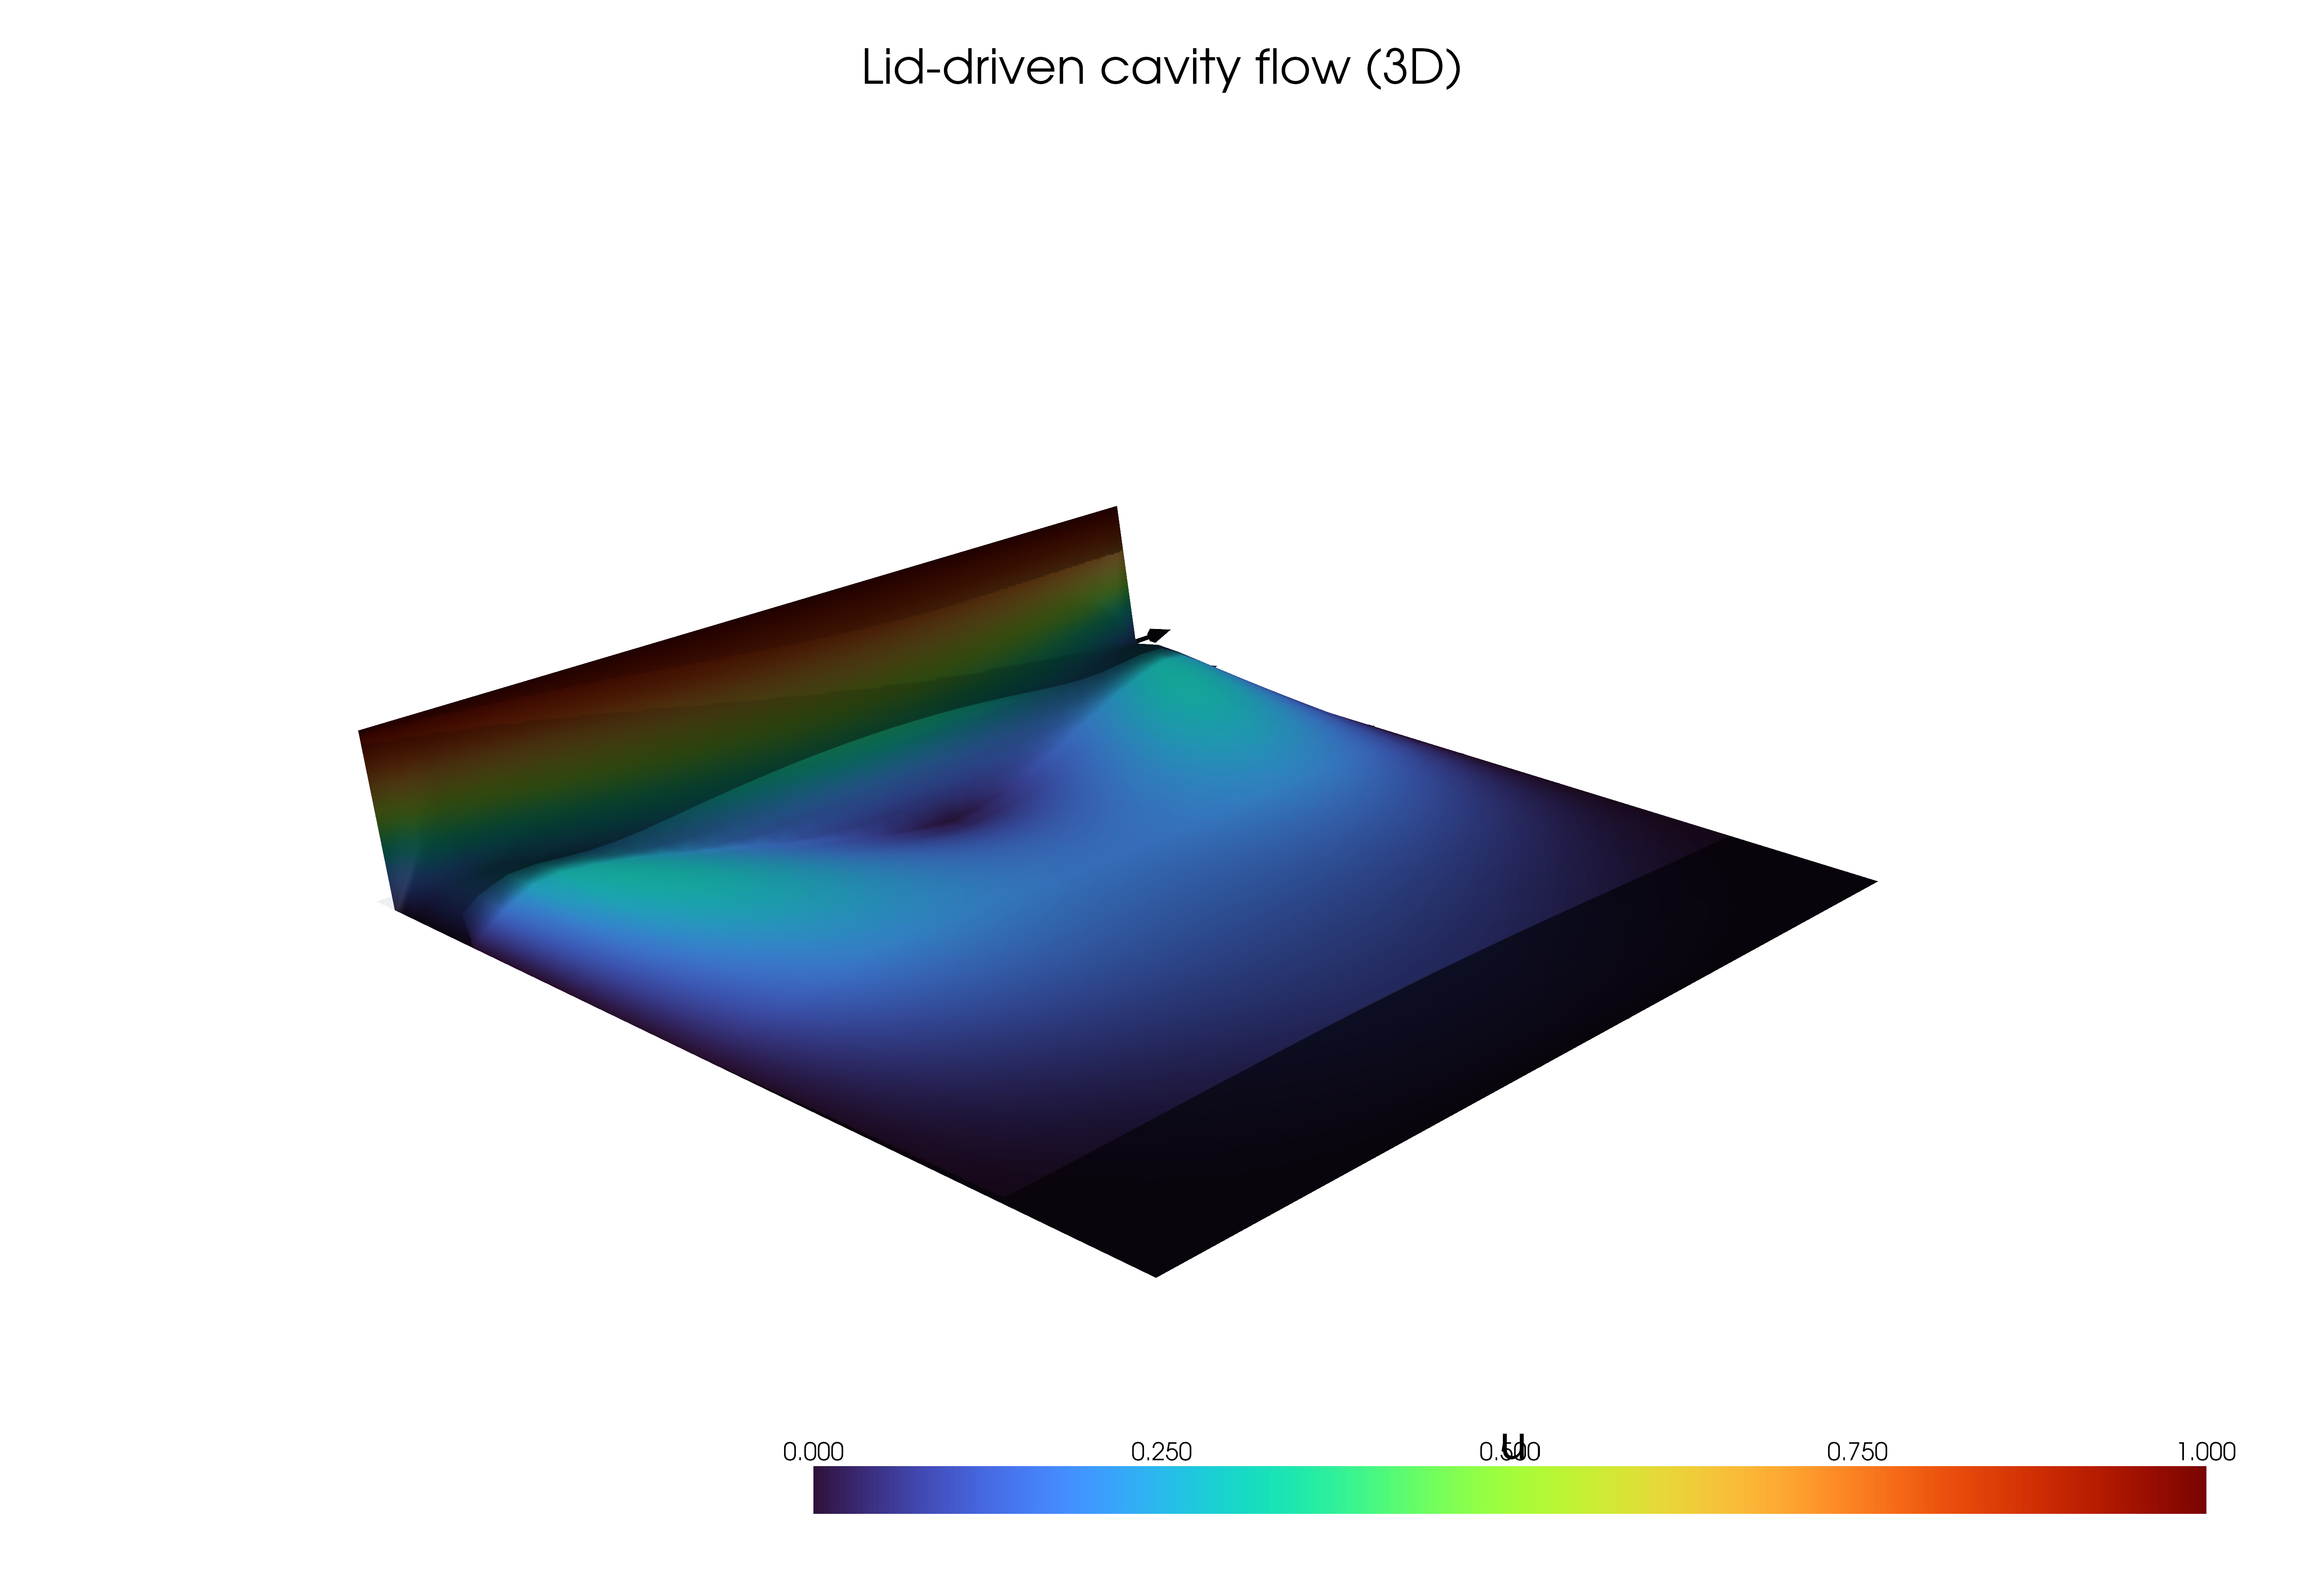
\includegraphics[width=0.495\textwidth]{stokes_cavity_3d.png}
\end{center}

\medskip
The computed cavity flow shown in the plane and as a surface.

\end{frame}

% ──────────────────────────────────────────────────────────────
\begin{frame}{Resources}

\textbf{Official:}
\begin{itemize}
    \item FEniCS Project: \url{https://fenicsproject.org}
    \item FEniCSx Tutorial: \url{https://jsdokken.com/dolfinx-tutorial/}
    \item Discourse Forum: \url{https://fenicsproject.discourse.group}
\end{itemize}

\bigskip

\textbf{Books \& Tutorials:}
\begin{itemize}
    \item Langtangen \& Logg, \emph{Solving PDEs in Python} (Springer, free PDF)
    \item The FEniCS Book (Springer, 2012) --- comprehensive reference
    \item FEniCS Tutorial: \url{https://fenicsproject.org/tutorial/}
\end{itemize}

\end{frame}

% ──────────────────────────────────────────────────────────────
\dividerframe{}{Questions?}

% ══════════════════════════════════════════════════════════════
%  BACKUP SLIDES
% ══════════════════════════════════════════════════════════════
\appendix

\begin{frame}[fragile]{Backup: complete Poisson code}

\begin{lstlisting}[basicstyle=\ttfamily\tiny]
from fenics import *
import matplotlib.pyplot as plt

mesh = UnitSquareMesh(8, 8)
V = FunctionSpace(mesh, 'P', 1)

u_D = Expression('1 + x[0]*x[0] + 2*x[1]*x[1]', degree=2)
bc = DirichletBC(V, u_D, 'on_boundary')

u = TrialFunction(V);  v = TestFunction(V)
f = Constant(-6.0)

a = dot(grad(u), grad(v)) * dx
L = f * v * dx

u_h = Function(V)
solve(a == L, u_h, bc)

error_L2 = errornorm(u_D, u_h, 'L2')
error_H1 = errornorm(u_D, u_h, 'H1')
print(f"L2 error: {error_L2:.6e}")
print(f"H1 error: {error_H1:.6e}")

plot(u_h); plt.colorbar(plot(u_h))
plt.savefig("poisson.png", dpi=150)
plt.show()
\end{lstlisting}

\end{frame}

\begin{frame}[fragile,shrink=4]{Backup: FEniCSx equivalent (DOLFINx)}

\begin{lstlisting}[basicstyle=\ttfamily\tiny]
import dolfinx, ufl
from dolfinx import fem, mesh
from mpi4py import MPI
import numpy as np

# Create mesh
msh = mesh.create_unit_square(MPI.COMM_WORLD, 8, 8)
V = fem.functionspace(msh, ("Lagrange", 1))

# Boundary condition
u_D = fem.Function(V)
u_D.interpolate(lambda x: 1 + x[0]**2 + 2*x[1]**2)
bdry_facets = mesh.locate_entities_boundary(
    msh, msh.topology.dim-1, lambda x: np.full(x.shape[1], True))
bc = fem.dirichletbc(u_D, fem.locate_dofs_topological(
    V, msh.topology.dim-1, bdry_facets))

# Variational problem
u = ufl.TrialFunction(V)
v = ufl.TestFunction(V)
f = fem.Constant(msh, -6.0)
a = ufl.dot(ufl.grad(u), ufl.grad(v)) * ufl.dx
L = f * v * ufl.dx

# Solve
problem = fem.petsc.LinearProblem(a, L, bcs=[bc])
u_h = problem.solve()
\end{lstlisting}

\small
Same concepts, slightly different API.

\end{frame}

\end{document}
